\documentclass[bachelor, substylefile=VolSU.rtx]{disser}

\usepackage[
  a4paper, mag=1000,
  left=3.0cm, right=1cm, top=2cm, bottom=2cm, headsep=0.7cm, footskip=1cm
]{geometry}

\usepackage[T2A]{fontenc}
\usepackage[utf8]{inputenc}
\usepackage[english, russian]{babel}
\usepackage{array}
\usepackage{amsmath, amssymb, amsfonts}
\usepackage{graphicx, epsfig}
\usepackage{enumitem} 
\usepackage{listings}
\usepackage{caption}
\usepackage{longtable}
\usepackage{multirow}
\usepackage{multicol}
\usepackage{makecell}

\usepackage{color}
\usepackage[colorlinks=false,linkcolor=blue,breaklinks]{hyperref}

\usepackage[citestyle=gost-numeric,style=gost-numeric,natbib=true,urldate=long, sorting=none,autolang=other]{biblatex}
\usepackage{csquotes}
\pagestyle{footcenter}
\chapterpagestyle{footcenter}

%для борьбы с переполнениями за счет разреженных слов в абзаце
\emergencystretch=5em

\graphicspath{{fig/}}
\addbibresource{Bib.bib}

\RequirePackage{caption}
\DeclareCaptionLabelSeparator{defffis}{ --- }
\captionsetup[figure]{justification=centering, labelsep=defffis}
\captionsetup[lstlisting]{
  justification=justified,
  singlelinecheck=false,
  labelsep=defffis,
  margin=2.5em
}
\captionsetup[table]{
  justification=justified,
  singlelinecheck=false,
  labelsep=defffis,
  margin=2.5em
}
%\captionsetup{justification=centering}
%\captionsetup{labelsep=defffis}


\begin{document}

\institution{Волгоградский государственный университет \\
Институт математики и информационных технологий \\
Кафедра информационных систем и компьютерного моделирования}

% Название практики и семестр
\title{Отчёт по производственной практике, научно-исследовательской работе}
\semester{второй семестр}
\topic{Автоматическое выявление дефектов в процессе 3D-печати}

\apname{А. В. Хоперсков}
% Автор
\author{Ешенко Даниил Ярославович}
\authorshort{Д.Я. Ешенко}
% Группа
\group{ИВТм-241}
\coursenum{09.04.01}
\course{Информатика и вычислительная техника}

% Руководитель практики (возможно Р. В. Щёлоков)
% \supervisor       {Р. В. Щёлоков}
% \supervisorstatus {к. ф.-м. н., доцент кафедры ИСКМ}

\supervisor       {Г. С. Иванченко}
\supervisorstatus {к. ф.-м. н., доцент кафедры ИСКМ}

% Организатор практики
\organizer        {А. С. Астахов}
\organizerstatus  {ст. преп. каф. ИСКМ}

% Научный консультант (опционально)
% \consultant       {И. О. Фамилия}
% \consultantstatus {должность, кафедра}

\city{Волгоград}
\date{\number\year}

\maketitle

\renewcommand\contentsname{Содержание}
\tableofcontents
\intro
За последние годы 3D-печать перешла от задач прототипирования к практическому применению в малосерийном производстве, учебных лабораториях и инженерных мастерских. Это стало возможным благодаря экономичности аддитивного подхода: он не требует оснастки при небольших партиях, уменьшает объём отходов по сравнению с традиционными методами и сокращает время изготовления изделий. Однако при переходе от единичных прототипов к серийному производству ключевым ограничением становится стабильность качества и точность результата.

В рамках данной работы рассматривается метод послойного наплавления (Fused Deposition Modeling, FDM). Изделие формируется последовательным нанесением расплавленного материала по слоям в соответствии с управляющей программой. Для FDM-процесса характерна высокая чувствительность к параметрам температуры, скорости печати и перемещений, охлаждения, адгезии первого слоя и к состоянию расходного материала. Отклонение даже одного из параметров может вызвать каскадное ухудшение качества изделия. Поэтому контроль процесса должен выполняться не постфактум, а непосредственно во время печати, когда еще возможно своевременно повлиять на ход задания.

Значимая часть отказов проявляется уже на ранних этапах печати и связана с нарушением устойчивости технологического процесса, что влияет на качество формируемого изделия. Если такие отклонения не обнаруживаются своевременно, последствиями становятся перерасход материала, потеря машинного времени, необходимость повторного запуска задания и рост эксплуатационной нагрузки на узлы принтера.

Дополнительной проблемой является простой оборудования между заданиями. На фермах 3D-принтеров и в учебно-производственных лабораториях операторы часто работают по графику~5/2, что формирует ночные и выходные периоды неполной загрузки. Частичный переход к дневным и ночным сменам позволяет сократить простой, но одновременно увеличивает затраты на персонал. Следовательно, для повышения общей эффективности необходимо снижать зависимость производственного цикла от постоянного присутствия оператора и переводить контроль печати в автоматизированный режим.

В рамках исследования разрабатывается 3D-принтер с функцией экспериментальной платформы и контуром раннего обнаружения дефектов во время печати. Этот контур включает видеонаблюдение зоны печати, обработку кадров, выявление и локализацию дефектов по изображению, а также передачу данных в управляющую логику принтера. Под реагированием подразумеваются заранее заданные действия, направленные на ограничение развития дефекта и снижение потерь материала и времени.

Полная автоматизация цикла, включая расширенную очередь заданий и автоматическое снятие изделий, рассматривается как перспектива дальнейшего развития. Однако в данной работе это не является основной целью. Тем не менее, основы для этого будут заложены уже сейчас.

Объектом исследования является процесс FDM-печати в условиях малосерийного производства и длительной эксплуатации оборудования. Предметом исследования являются методы и программно-аппаратные средства раннего обнаружения дефектов 3D-печати по данным видеоконтроля, а также способы их интеграции в контур управления принтером для оперативного принятия решений.

Практическая значимость работы состоит в том, что полученная первая версия системы задаёт основу для перехода от ручного контроля к контролю в процессе печати. Ранняя фиксация отклонений позволяет сократить потери материала и времени, а также формирует архитектуру, пригодную для дальнейшего расширения функций автономной работы.

Актуальность работы определяется тем, что небольшие нарушения режима FDM-печати приводят к браку и повторным запускам, увеличивая потери материала и времени и снижая загрузку оборудования. В таких условиях автоматическое обнаружение и локализация дефектов с реакцией в ходе печати является практической и научно-технической задачей. На момент написания работы в открытых источниках и на российском рынке не выявлено распространённого решения для FDM, которое встраивается в контур управления принтером и обеспечивает раннее обнаружение дефектов по видеопотоку с заранее заданными сценариями реакции. При этом существуют зарубежные системы мониторинга со схожей целью (в том числе с функциями обнаружения отказов с применением искусственного интеллекта (ИИ) и действиями вроде уведомления или паузы печати), однако их принципы работы и степень интеграции с управляющей логикой отличаются от рассматриваемого в данной работе подхода. Поэтому разработка и экспериментальная проверка первой версии системы для FDM-печати с функцией раннего обнаружения дефектов и реакцией на них является актуальной задачей, которая может внести вклад в повышение эффективности и качества 3D-печати.

Целью данной работы является разработка и экспериментальная проверка первой версии 3D-принтера с системой раннего обнаружения дефектов в процессе печати и механизмом своевременного реагирования. Для достижения поставленной цели необходимо решить следующие задачи:
\begin{enumerate}
\item проанализировать технологический цикл FDM-печати и выделить дефекты, критичные для раннего обнаружения;
\item сформировать требования к архитектуре программно-аппаратного контура, включающего принтер, камеру, обработку данных и подсистему управления;
\item организовать подготовку и разметку визуальных данных для обучения и проверки модели обнаружения дефектов;
\item разработать модель обнаружения дефектов для целевых классов;
\item реализовать интеграцию модуля обнаружения в рабочий цикл принтера и настроить сценарии своевременного реагирования на выявленные отклонения;
\item провести экспериментальную проверку работоспособности первой версии на серии печатей и зафиксировать ограничения текущей реализации;
\item определить направления развития решения, включая расширение автономности цикла и развитие очереди заданий.
\end{enumerate}

\chapter{Анализ технологического процесса 3D-печати и причин возникновения дефектов}

\section{Технология послойного наплавления: принципы, ограничения и критичные параметры процесса}

В данной работе рассматривается технология печати методом послойного наплавления, для которой разрабатывается контур мониторинга и раннего обнаружения отклонений. Метод послойного наплавления (Fused Deposition Modeling, FDM)~-- аддитивный метод, при котором полимерная нить подается в нагревательный блок, расплавляется и через сопло наносится слоями, формируя геометрию изделия~\cite{лысыч2014области}.

Схема устройства FDM-принтера приведена на рисунке~\ref{fig:FDM}.

\begin{figure}[h!]
\centering
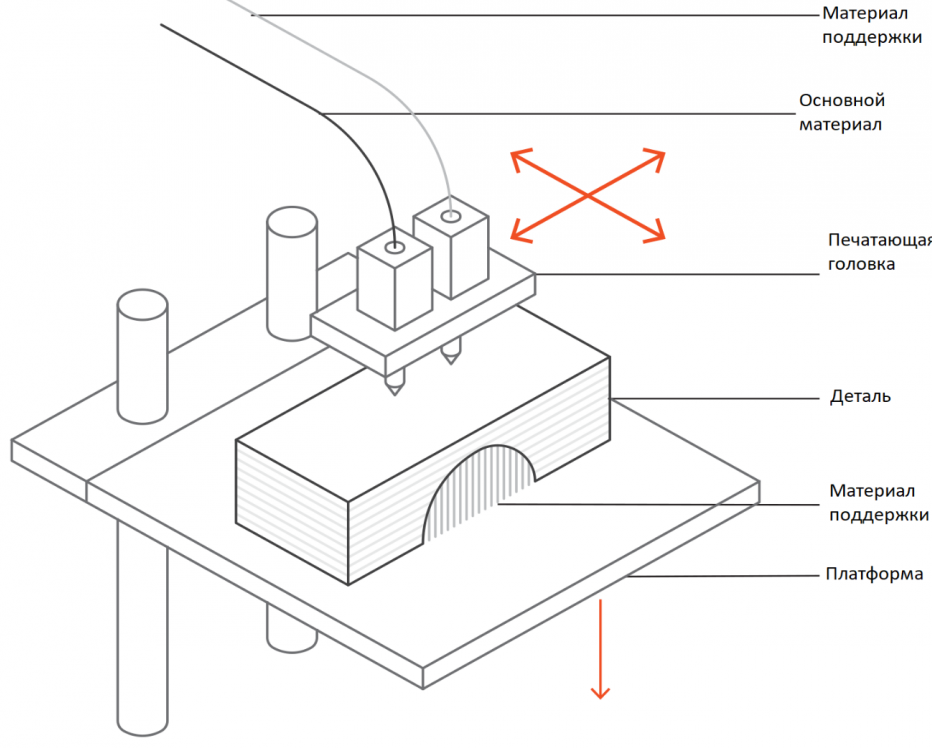
\includegraphics[width=0.75\hsize]{fig/FDM.png}
\caption{Схема устройства FDM-принтера}
\label{fig:FDM}
\end{figure}

Технологический цикл метода включает подготовку модели, формирование управляющей траектории и последовательное построение изделия слоями. Качество результата в таком процессе определяется не одним параметром, а совокупностью факторов, связанных с материалом, состоянием оборудования, условиями среды и корректностью цифровой подготовки задания.

С практической точки зрения дефекты FDM-печати целесообразно рассматривать как следствие нарушения устойчивости процесса. Если в одном из звеньев технологической цепочки возникает отклонение, оно переносится на последующие слои и может усиливаться по мере роста изделия. Поэтому анализ причин дефектов должен выполняться комплексно, а не только через локальные корректировки отдельных настроек.

Важным элементом процесса является филамент -- полимерный расходный материал в виде непрерывной нити, который подается в экструдер, расплавляется и формирует дорожки слоя. Свойства филамента непосредственно влияют на стабильность экструзии, характер межслойного сцепления и повторяемость геометрии. Даже при исправной механике принтера нестабильное качество материала способно привести к систематическим отклонениям результата.

Среди типовых источников проблем со стороны материала выделяются неоднородность состава, отклонения диаметра нити, повышенная влажность и наличие посторонних включений. Неоднородность расплава вызывает неравномерную подачу, что отражается на форме дорожек и точности контуров. Влажный материал при нагреве может давать нестабильную экструзию и ухудшать качество поверхности, а твердые включения повышают риск частичных засоров и ускоренного износа сопла.

На итог печати влияет не только химический состав филамента, но и его физическое состояние в момент использования. Перегибы нити, повышенное трение в тракте подачи и нестабильная намотка катушки создают дополнительные возмущения потока материала. В результате возникают локальные нарушения структуры слоя, которые визуально проявляются как ухудшение геометрии, неоднородность поверхности и снижение эксплуатационной пригодности детали.

Отдельную группу причин образуют факторы оборудования и кинематики: люфты, износ механических узлов, нестабильность перемещений, загрязнение рабочих элементов и недостаточная повторяемость позиционирования. Эти отклонения не всегда приводят к мгновенному браку, однако постепенно формируют накопительный эффект, при котором небольшие погрешности первых слоев переходят в заметные дефекты на более поздних стадиях печати.

Существенное влияние оказывают и внешние условия выполнения задания. Колебания температуры, локальные потоки воздуха и нестабильность теплообмена в рабочей зоне изменяют режим формирования слоя и межслойного контакта. Для длительных заданий это особенно критично, поскольку продолжительность процесса повышает чувствительность к малым, но систематическим воздействиям среды.

Причины дефектов в FDM-печати удобно группировать по четырем блокам: материал, оборудование, цифровая подготовка и внешние условия. Такая структура позволяет связать наблюдаемое отклонение с вероятным источником и выбрать корректирующее действие на уровне причины, а не только на уровне внешнего симптома. Для задач автоматизированного контроля это принципиально, так как повышает достоверность диагностики и снижает риск повторения дефекта в следующих циклах печати.

Таким образом, филамент следует рассматривать как один из ключевых факторов устойчивости FDM-процесса наряду с состоянием принтера и условиями эксплуатации. Комплексный учет этих факторов формирует основу для раннего обнаружения отклонений и для построения системы, способной своевременно реагировать на признаки ухудшения качества печати. Далее рассматриваются основные классы дефектов FDM-печати.

\section{Классы дефектов печати и факторы их возникновения в реальных условиях эксплуатации}

В реальных условиях эксплуатации дефекты FDM-печати формируются не как изолированные события, а как результат совокупного влияния материала, оборудования, подготовленного задания и внешней среды. Для практической задачи мониторинга важно перечислить возможные отклонения. Отдельно необходимо выделить классы, которые одновременно являются критичными для процесса и устойчиво наблюдаются по визуальным признакам во время печати.

С инженерной точки зрения дефекты целесообразно разделять по последствиям: ухудшение геометрии и внешнего вида изделия, снижение прочности, срыв текущего задания и риск повреждения узлов принтера. Для разработки системы автоматического обнаружения приоритет получают состояния, при которых задержка реакции приводит к наибольшим потерям материала, времени и ресурса оборудования.

В данной работе рассматривается широкий набор возможных отклонений. В качестве целевых классов для автоматического распознавания выбраны четыре наиболее критичных дефекта: растрескивание, отлипание модели от стола, дефект типа «спагетти» и смещение слоев. Такой выбор позволяет сосредоточить обучение модели на сценариях с максимальным практическим эффектом от раннего обнаружения.

Растрескивание отражает нарушение целостности изделия и связано с потерей межслойной прочности. На практике этот дефект проявляется при неблагоприятном тепловом режиме, неравномерном охлаждении и недостаточной адгезии между слоями. Даже локальные трещины ухудшают эксплуатационные свойства детали и часто делают результат печати непригодным для целевого применения.

Отлипание модели от стола является критическим дефектом начальной стадии, поскольку нарушает базовую геометрию всего дальнейшего построения. Причинами обычно выступают нестабильная адгезия первого слоя, состояние рабочей поверхности и совокупность факторов, влияющих на удержание детали в процессе роста высоты. При развитии этого отклонения печать теряет воспроизводимость и переходит в аварийный режим.

Дефект типа «спагетти» возникает при потере корректного контакта экструдируемого материала с моделью, когда подача пластика продолжается, но формирование слоя уже нарушено. В результате материал накапливается в виде хаотичных нитей, а задание фактически выполняется вхолостую. Этот сценарий быстро увеличивает расход материала и машинного времени, а также затрудняет последующее восстановление рабочего состояния принтера.

Смещение слоев относится к дефектам, при которых траектория укладки материала сдвигается относительно ранее сформированной части изделия. Визуально это проявляется в виде ступенчатого смещения контуров и несоосности стенок, что приводит к искажению геометрии и снижению пригодности детали. Причинами смещения обычно являются пропуски шагов приводов, перегрузка кинематики, недостаточное натяжение ремней, заедания механики или столкновения с деформациями изделия; поэтому данный дефект рассматривается как приоритетный для раннего выявления и своевременного реагирования.

Важной особенностью реальной эксплуатации является динамика развития дефектов: например, отлипание может привести к «спагетти», а нарушения работы приводов и кинематики — к смещению слоев. Следовательно, система контроля должна учитывать динамику процесса и обнаруживать признаки отклонений на ранней стадии, до перехода в более тяжелый сценарий.

Таким образом, в рамках работы основное внимание сосредоточено на четырех целевых классах дефектов: растрескивание, отлипание, «спагетти» и смещение слоев. На этих группах формируется разметка данных и выполняется обучение нейросетевой модели обнаружения, поскольку именно они имеют наибольшее значение для устойчивости печати и безопасности эксплуатации оборудования.

Сводная характеристика приоритетных дефектов для раннего обнаружения приведена в таблице~\ref{table:defects_priority}.

\begin{table}[ht]
\caption{Сводная характеристика приоритетных дефектов для раннего обнаружения}
\label{table:defects_priority}
\scriptsize
\renewcommand{\arraystretch}{1.05}
\setlength{\tabcolsep}{3pt}
\centering
\begin{tabular}{|>{\raggedright\arraybackslash}m{70pt}|>{\raggedright\arraybackslash}m{86pt}|>{\raggedright\arraybackslash}m{88pt}|>{\raggedright\arraybackslash}m{58pt}|>{\raggedright\arraybackslash}m{86pt}|}
\hline
Дефект & Ранние визуальные признаки & Влияние на процесс & Приоритет реагирования & Базовое действие системы \tabularnewline
\hline
Растрескивание & Трещины, расхождение слоев, нарушение поверхности & Потеря прочности, риск непригодности детали & Высокий & Фиксация события, уведомление, контроль динамики \tabularnewline
\hline
Отлипание модели от стола & Смещение модели, потеря контакта первого слоя со столом & Срыв геометрии, потеря воспроизводимости печати & Критический & Немедленная пауза и остановка при подтверждении отклонения \tabularnewline
\hline
Дефект типа «спагетти» & Хаотичные нити пластика вне контура модели & Бесполезный расход материала, потеря машинного времени & Критический & Остановка задания, уведомление, подготовка к перезапуску \tabularnewline
\hline
Смещение слоев & Ступенчатый сдвиг контуров, несоосность слоев & Искажение геометрии, риск непригодности детали & Высокий & Фиксация события, уведомление, пауза при подтверждении отклонения \tabularnewline
\hline
\end{tabular}
\end{table}

Далее рассматривается влияние выделенных дефектов на качество изделий, расход материала и надежность оборудования.

\section{Влияние дефектов на качество изделий, расход материала и надежность оборудования}

Анализ последствий дефектов в процессе~3D-печати необходим для оценки устойчивости технологического цикла и эффективности эксплуатации оборудования. Если отклонения не выявляются на ранней стадии, они переходят из локальной проблемы качества в фактор, влияющий на весь производственный контур. В результате возрастает доля незавершенных заданий, снижается предсказуемость результата и увеличиваются совокупные издержки выполнения печати.

Первый уровень последствий связан с качеством готового изделия. Дефекты нарушают геометрию детали, равномерность структуры и целостность межслойных связей, из-за чего итоговый объект может не соответствовать требованиям по размерам и форме. Для прикладных задач это означает снижение повторяемости результата: даже при одинаковом задании итоговые характеристики деталей становятся нестабильными, что усложняет последующую сборку и использование изделий по назначению.

Второй уровень последствий проявляется в эксплуатационной пригодности изготовленной детали. При наличии дефектов снижается фактическая прочность изделия, ухудшается устойчивость к рабочим нагрузкам и повышается вероятность отказа в процессе применения. Даже если деталь сохраняет внешний вид, внутренние нарушения структуры могут ограничивать срок службы и требовать повторного изготовления, что снижает практическую ценность результата печати.

Третий уровень связан с расходом материалов и затратами машинного времени. Любое прерванное или некачественное задание приводит к прямым потерям филамента, а повторный запуск увеличивает длительность выполнения одной и той же технологической операции. При серийных задачах такие потери накапливаются, формируя дополнительную нагрузку на оператора и уменьшая фактическую производительность печатного контура.

Отдельно необходимо учитывать влияние дефектов на надежность оборудования. При работе в условиях отклонений возрастают механические и тепловые нагрузки на узлы подачи материала и печатающую головку, увеличивается частота обслуживающих операций и сокращаются интервалы стабильной работы без вмешательства. Это приводит к ускоренному износу отдельных компонентов, повышает вероятность внеплановой остановки и увеличивает трудоемкость восстановления рабочего состояния принтера.

Существенным последствием является рост простоев оборудования. Время, затрачиваемое на остановку задания, диагностику причин, очистку рабочей зоны, повторную подготовку поверхности и перезапуск печати, исключает принтер из полезного производственного цикла. При регулярном повторении таких сценариев снижается пропускная способность системы, а график выполнения заданий становится менее управляемым и менее прогнозируемым.

В совокупности дефекты выступают не только как показатель качества отдельной детали, но и как фактор технико-экономической эффективности всей системы~3D-печати. Их влияние одновременно затрагивает качество продукции, стабильность эксплуатации оборудования и себестоимость выполнения задач. Следовательно, оценка и раннее обнаружение отклонений должны рассматриваться как обязательный элемент управления процессом, а не как дополнительная операция контроля после завершения печати.

С учетом указанных последствий в рамках работы приоритет отдается четырем группам дефектов, оказывающим наибольшее влияние на устойчивость цикла и безопасность эксплуатации: растрескивание, отлипание модели от стола, дефект типа «спагетти» и смещение слоев. Концентрация обучения нейросетевой модели на этих группах повышает практическую значимость автоматического контроля. За счет такого фокуса система обеспечивает более полезный эффект от раннего реагирования.

\section{Методы мониторинга процесса печати и подходы к раннему обнаружению отклонений}

Мониторинг процесса~3D-печати является ключевым условием устойчивой работы производственного контура, поскольку отклонения формируются во времени и накапливаются от слоя к слою. Если признаки нарушения фиксируются поздно, система теряет возможность локального вмешательства и переходит к затратному сценарию полного перезапуска задания. По этой причине раннее обнаружение рассматривается как технологическая функция управления, а не как вспомогательный этап контроля готовой детали.

Базовым и наиболее распространенным подходом остается ручной визуальный контроль оператором. Его сильной стороной является простота внедрения и возможность оперативной качественной оценки состояния процесса без сложной инфраструктуры. Однако такой метод зависит от непрерывного присутствия человека, имеет выраженную субъективность и не обеспечивает одинаковую скорость реакции в длительных или параллельных циклах печати.

Альтернативой служит порогово-правиловый контроль, основанный на анализе состояния процесса и сервисных сигналов. Этот подход позволяет формализовать базовые критерии нормальной работы и автоматически фиксировать отклонения по заранее заданным условиям. Его ограничение состоит в том, что правила хорошо покрывают типовые режимы, но хуже адаптируются к нестандартным визуальным сценариям, где проблема проявляется раньше, чем становится доступной в виде явного дискретного события.

Третьим направлением является алгоритмический анализ изображений с применением методов машинного обучения, ориентированных на распознавание аномалий в зоне печати. Такой подход снижает зависимость от оператора и позволяет выявлять визуальные признаки отклонений на стадии их раннего формирования. Вместе с тем его качество определяется полнотой и репрезентативностью обучающих данных, а при недостаточной калибровке критериев возможны ложные срабатывания и пропуски событий.

Сравнение указанных подходов показывает, что изолированное применение любого из них создает эксплуатационные ограничения. Ручной контроль недостаточно масштабируем, порогово-правиловый чувствителен к полноте формализованных условий, а алгоритмический анализ требует устойчивого контура валидации результатов. Следовательно, для реальных условий~3D-печати целесообразно использовать комбинированную схему, в которой сильные стороны одного метода компенсируют ограничения другого.

В рамках данной работы обосновывается гибридный подход к мониторингу: непрерывное визуальное наблюдение за зоной печати сочетается с алгоритмическим анализом признаков отклонений и с контролем состояния технологического процесса. Такое объединение повышает достоверность диагностического решения, поскольку итоговая оценка опирается не на один источник данных, а на согласование нескольких независимых признаков. В результате система получает возможность фиксировать отклонения раньше и уменьшать вероятность развития дефекта до критической стадии.

Для практического применения выбран комбинированный сценарий реакции на события мониторинга. На первом уровне выполняются фиксация инцидента и уведомление оператора, что обеспечивает прозрачность и последующую проверяемость принятых решений. На втором уровне, при подтверждении критичности отклонения, система инициирует управляющее воздействие в виде паузы или остановки процесса, ограничивая потери материала, машинного времени и риска для оборудования.

Таким образом, мониторинг в данной работе рассматривается как связанный контур наблюдения, анализа и управляющего реагирования, ориентированный на раннее обнаружение отклонений в процессе~3D-печати. Применение гибридной схемы позволяет снизить долю неуспешных заданий и сократить простои за счет своевременного вмешательства. Полученные положения формируют методическую основу для дальнейшего архитектурного обоснования аппаратно-программного комплекса контроля процесса печати в следующей главе.

\chapter{Выбор программных и аппаратных средств для реализации приложения}

Для того чтобы создать Android-приложение, способное обнаруживать дефекты 3D-печати, необходимо комплексное решение, объединяющее знания в области материаловедения, машинного зрения и мобильной разработки. Прежде всего, следует провести анализ и классификацию наиболее распространённых дефектов, таких как недостаточная адгезия первого слоя, деформация, перегрев, недостаточное охлаждение, а также «спагетти» \cite{заикин2023проектирование}. Именно эти проблемы чаще всего возникают у новичков, и их распознавание может стать отправной точкой для дальнейшей оптимизации процесса печати.

Затем следует создать алгоритмы компьютерного зрения, которые будут точно распознавать дефекты на основе изображений, получаемых с камеры Android-устройства. Для этого можно применить современные методы обработки изображений и сверточные нейронные сети, специально настроенные на задачу сегментации и классификации дефектов \cite{измайлов2020анализ}.

Следует уделить внимание созданию интуитивно понятного пользовательского интерфейса, который позволит оперативно получать обратную связь о качестве печати и своевременно корректировать настройки 3D-принтера.

\section{Выбор средств для аннотирования изображений и обучения нейросети}

Так как задача создания приложения для обнаружения дефектов требует оперативной и точной идентификации отклонений в режиме реального времени, оптимальным выбором является использование архитектуры YOLO (You Only Look Once, что в переводе с английского означает «ты смотришь только один раз»). YOLO -- это сверточная нейронная сеть, которая обрабатывает изображение за один проход, одновременно определяя местоположение и тип объектов. Такой подход обеспечивает высокую скорость работы и точность детекции, что особенно важно для мобильных решений \cite{брехт2022применение}.

Например, в отличие от двухступенчатых методов, таких как Faster R-CNN (Faster Region-based Convolutional Neural Network -- Быстрая Региональная Сверточная Нейронная Сеть), где сначала генерируются регионы интереса, а затем происходит их классификация, YOLO обрабатывает изображение целиком за один проход. Такой подход позволяет достигать скоростей до 45–155 кадров в секунду, что особенно важно для систем, работающих в режиме реального времени (real-time systems), например, для мобильных приложений по обнаружению дефектов или систем видеонаблюдения.

Еще одним примером является сравнение с архитектурой SSD (Single Shot MultiBox Detector, «Однокадровый мультибокс-детектор»). Несмотря на то, что SSD также реализует детекцию объектов за один проход, YOLO часто демонстрирует более высокую производительность на сложных изображениях благодаря более глубокому и оптимизированному сверточному базису и улучшенной стратегии прогнозирования ограничивающих рамок \cite{lishchenko2022online}.

Кроме того, благодаря своей архитектуре YOLO может эффективно интегрироваться в облачные и мобильные приложения, что делает её универсальным инструментом для широкого спектра сценариев использования.

Для аннотирования изображений был выбран Roboflow -- это облачная платформа для управления наборами данных, разметки и обучения моделей компьютерного зрения. Она предоставляет удобный RESTful API (интерфейс программирования приложений, построенный на принципах архитектуры REST, когда запросы отправляются по протоколу HTTP) и библиотеку для Python. Это упрощает интеграцию процесса подготовки данных и обучения нейросетей в различные приложения.

Основное преимущество Roboflow заключается в том, что она позволяет легко загружать, аннотировать и преобразовывать изображения, а также применять аугментацию -- метод искусственного увеличения объёма обучающего набора данных путём внесения случайных изменений, таких как повороты, масштабирование и изменение яркости \cite{kukartsev2024deep}. Такой подход значительно ускоряет подготовку набора данных для обучения моделей, обеспечивая более высокое качество финальных результатов.

Roboflow, благодаря своей облачной инфраструктуре, может работать с большими объёмами данных, что крайне важно для обучения сложных моделей. Это позволяет выполнять цикл обучения быстро и оптимизировать параметры модели.

После обучения модель можно развернуть и использовать через API. Это даёт возможность быстро внедрять системы обнаружения объектов в мобильные приложения или промышленные системы мониторинга\cite{богданов2019технология}.

\section{Выбор интегрируемой среды разработки для создания мобильного приложения на Android}

При разработке мобильных приложений для Android выбор оптимальной интегрированной среды разработки (Integrated Development Environment, IDE) -- это один из самых важных этапов. От этого выбора зависит, насколько эффективно будет возможно писать, отлаживать и тестировать код.

После тщательного анализа доступных инструментов, таких как Eclipse с плагином Android Development Tools (ADT -- инструменты разработки для Android) и IntelliJ IDEA, особое внимание было уделено Android Studio\cite{kocakoyun2017developing}. Эта среда разработки, являющаяся официальным продуктом компании Google, обеспечивает своевременное обновление и полную совместимость с последними версиями Android Software Development Kit (SDK — набор средств разработки программного обеспечения), что гарантирует доступ к современным функциям и возможностям, необходимым для создания качественных приложений.

Одним из главных преимуществ Android Studio является интеграция с системой сборки Gradle -- мощным инструментом автоматизации, который помогает управлять зависимостями проекта и оптимизировать процесс сборки. Эта интеграция значительно ускоряет цикл разработки, а также способствует повышению стабильности и производительности конечного продукта\cite{craig2015learn}.

После изучения различных инструментов был сделан выбор в пользу Android Studio\cite{zapata2016android}. Поскольку и Android, и Android Studio являются официальными продуктами компании Google, эта среда разработки регулярно обновляется и полностью совместима с последними версиями операционной системы Android.
\chapter{Проектирование и разработка мобильного приложения на Anroid}

\section{Планирование и анализ рабочего процесса}

Диаграмма Ганта помогает распределить планируемое время по конкретным задачам. В данной работе составлена диаграмма Ганта, состаящая из 5 этапов, идущими последовательно. Представлена она на рисунке \ref{fig:гант} и составлена на период с 30 сентября 2024 года по 27 января 2025 года. 

\begin{figure}[h!]
\begin{center}
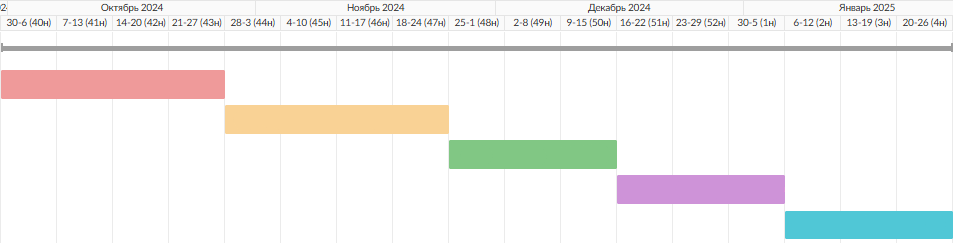
\includegraphics[width=1\hsize]{fig/гант.png}
\caption{Диаграмма Ганта}\label{fig:гант}
\end{center}
\end{figure}

На данной диаграмме красным цветом (первая строка) обозначена задача изучения предметной области (теоретических материалов). Желтым (вторая строка) -- формирование набора данных и обучение нейронной сети. Зеленым (третья строка) -- проектирование приложения и разработка серверной части. Фиолетовым цветом (четвертая строка) -- разработка интерфейса для мобильного приложения. Голубым (пятая строка) -- анализ полученных результатов, подведение итогов. 

По данной диаграмме больше всего времени планируется выделить на формирование набора данных (разметку, аннотирование и аугментацию изображений) и обучение нейронной сети, так как для качественного распознавания, нужно максимально точно разметить границы на каждом изображении. Кроме того, обучение нейросети, основанной на архитектуре YOLO с использованием аугментации, требует значительных временных и вычислительных ресурсов. Этап ознакомления с теоретическими материалы данной области также занимает много времени, поскольку, как описывалось в актуальности работы, аналогов такой программы пока не выпущено.

Каждой из задач требуется уделить особое внимание, поскольку все они могут повлиять на конечный результат. 

\section{Формирование набора данных, аннотирование и аугментация изображений}

Для создания качественного набора данных был проведен поиск изображений в открытых источниках, тематических группах и датасетах. Отбирались изображения с дефектами, описанными в первой главе. Найденные изображения загружались на платформу Roboflow в отдельный проект.

При подготовке данных особое внимание уделялось точной разметке изображений. Важно, чтобы границы дефектов соответствовали реальным размерам и не перекрывались. Если ограничивающая рамка больше реального дефекта, это может исказить представление о дефекте и затруднить обучение модели. Если рамки пересекаются, один и тот же дефект может быть отмечен несколькими рамками, что приводит к дублированию информации и искажению размеров. 

Данные ошибки снижают значение метрики Intersection over Union (пересечение над объединением -- показатель, характеризующий степень совпадения предсказанной рамки с истинной), что негативно сказывается на оценке качества обнаружения. Неточности в разметке могут привести к переобучению, когда модель становится чувствительной к шуму и не способна обобщать информацию на новые изображения.

На рисунках \ref{fig:big} и \ref{fig:Granitsi} продемонстрированы неправильно расставленные границы дефектов.

\begin{figure}[h!]
  \begin{minipage}[b]{0.45\hsize}
    \centering
    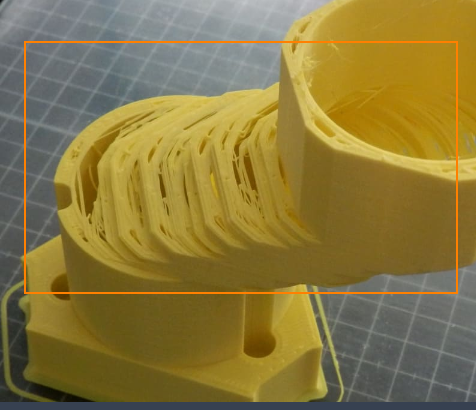
\includegraphics[width=\hsize]{fig/big.png}
    \caption{Слишком большие границы дефекта}
    \label{fig:big}
  \end{minipage}
  \hfill
  \begin{minipage}[b]{0.45\hsize}
    \centering
    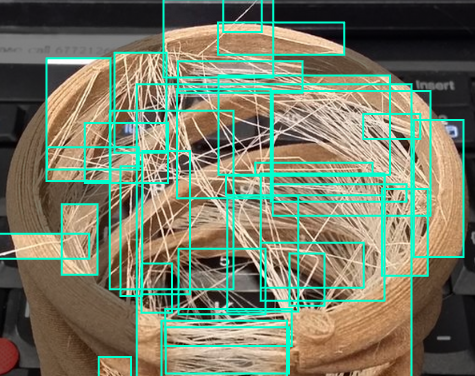
\includegraphics[width=\hsize]{fig/Granitsi.png}
    \caption{Границы дефектов перекрывают друг-друга}
    \label{fig:Granitsi}
  \end{minipage}
\end{figure}

Избегая данных ошибок при разметке, необходимо вручную разметить каждое изображение в наборе, выделяя дефекты разным цветом. Платформа Roboflow предлагает автоматическую разметку, но в данной задаче её точность оказалась недостаточной. Также Roboflow позволяет аннотировать изображения не только с помощью ограничивающих прямоугольников, но и полигонов, которые обеспечивают более точное описание контуров объектов. Изначально изображения были размечены с использованием полигонов, но их точность оказалась низкой, поэтому использовался классический вариант с прямоугольниками. Этот подход позволяет более стабильно и точно выделять дефекты, что является ключевым фактором для успешного обучения модели компьютерного зрения.

\section{Проектирование приложения и его серверной части}

Чтобы выполнять задачу обнаружения дефектов 3D-печати, требуются достаточно сложные вычислительные задачи. Чтобы снизить требования к Android-устройству было принято решение выполнять все вычисления и обработку изображений на серверной части. 

Централизованная серверная обработка обеспечивает безопасность и контроль качества, упрощает мониторинг и обновление моделей, а также снижает вероятность ошибок, связанных с разнообразием условий эксплуатации на конечных устройствах.

Серверная часть представляет собой веб-сервис, разработанный на языке Python с использованием микрофреймворка Flask (Flask --- фреймворк для создания веб-приложений на Python). Данный сервер предназначен для обработки изображений, получаемых через HTTP-запросы, и последующего обнаружения дефектов 3D-печати с использованием обученной модели, доступной через облачный API Roboflow.

Работа сервера начинается с инициализации приложения Flask, что позволяет ему принимать запросы от клиентов. Для обеспечения возможности взаимодействия с приложениями, работающими на других доменах или устройствах, используется библиотека flask cors (Cross-Origin Resource Sharing -- механизм, позволяющий осуществлять запросы с других источников).

После запуска сервера выполняется подключение к рабочему пространству и загрузка модели, обученной для обнаружения дефектов. Если модель не загружается корректно, сервер регистрирует ошибку, что позволяет избежать дальнейших сбоев при обработке запросов. Весь код серверной части представлен в приложении: Листинг \ref{ls:a:01}.

Основной функционал сервера реализован в эндпоинте (точке входа). Этот эндпоинт принимает POST-запросы, содержащие изображение и уникальный идентификатор устройства (device id). После проверки корректности полученного файла (например, формат файла должен быть JPG, JPEG или PNG) изображение сохраняется в папку uploads с уникальным именем, сформированным на основе device id и случайного уникального идентификатора (UUID -- Universally Unique Identifier, универсальный уникальный идентификатор).

После того как изображение было сохранено, сервер отправляет его в Roboflow для анализа с помощью метода predict, установив минимальный уровень доверия (confidence threshold) и параметр перекрытия (overlap). Минимальный уровень доверия представляет собой границу, ниже которой предсказанные объекты исключаются из рассмотрения. Это означает, что если модель не уверена в наличии дефекта с вероятностью выше установленного значения, то её предсказание не принимается во внимание. Такой подход позволяет уменьшить количество ошибочных срабатываний и повысить точность конечных результатов.

Параметр перекрытия определяет, насколько допустимо пересечение ограничивающих рамок различных предсказаний. Если эти рамки накладываются друг на друга на определённую величину, установленную параметром перекрытия, они могут быть объединены или одна из них может быть исключена как дублирующая. Такой подход позволяет более точно и однозначно выделить области, где были обнаружены дефекты.

Полученный результат содержит координаты ограничивающих рамок и метки обнаруженных дефектов. С использованием библиотеки OpenCV (Open Source Computer Vision Library -- библиотека для компьютерного зрения) изображение аннотируется: на него накладываются прямоугольники и текстовые метки, что визуально выделяет обнаруженные дефекты.

Аннотированное изображение сохраняется в папке «output». Сервер отправляет клиенту JSON-ответ, который включает в себя список обнаруженных дефектов и URL аннотированного изображения. 

Android-часть проекта -- клиентское приложение для обнаружения дефектов 3D-печати, разработанное с использованием языка программирования Kotlin и платформы Android. Архитектура приложения разделена на несколько ключевых компонентов, каждый из которых выполняет свою роль и обеспечивает взаимодействие с серверной частью для обработки изображений.

Файл MainActivity.kt -- это основа приложения. Он отвечает за первоначальную настройку интерфейса, проверку условий первого запуска, а также за скрытие панели управления, которая содержит элементы навигации. Кроме того, MainActivity.kt настраивает обработчики нажатий, позволяя пользователю легко перемещаться между экранами.

Файл OtherActivity.kt отвечает за выбор изображения и его предварительный просмотр. При помощи механизма выбора контента приложение получает URI выбранного изображения. Библиотека Glide (инструмент для быстрой загрузки и отображения изображений) используется для отображения выбранного изображения в интерфейсе. Дополнительно реализован процесс преобразования URI в локальный файл с использованием стандартных средств языка Java, что необходимо для дальнейшей передачи изображения на сервер.

Общение с серверной частью организовано с помощью RetrofitClient.kt, объекта, который настраивает клиент для выполнения HTTP-запросов посредством библиотеки Retrofit (фреймворк для работы с RESTful API -- интерфейс программирования приложений, основанный на архитектурном стиле REST). В конфигурации используется OkHttpClient (библиотека для работы с HTTP-запросами) с добавленным HttpLoggingInterceptor (инструмент для логирования HTTP-запросов), что позволяет отслеживать и отлаживать сетевую активность. Этот компонент устанавливает базовый URL сервера, задаёт таймауты соединения и чтения, а также создаёт экземпляр интерфейса ApiService.

Файл CustomHttpClient.java предоставляет дополнительные параметры настройки OkHttpClient, аналогичные тем, что используются в RetrofitClient.kt. Основное внимание уделяется расширенным настройкам таймаутов и логирования, что позволяет повысить стабильность и упростить отладку сетевых операций.

Интерфейс ApiService.kt описывает конечную точку API для загрузки изображения. С использованием аннотаций Retrofit (например, Multipart и POST) определяется тип запроса, позволяющий передавать изображение в формате multipart/form-data вместе с текстовым параметром, представляющим уникальный идентификатор устройства. 

При использовании данного формата тело запроса разбивается на несколько частей, каждая из которых отделена специальной строкой, называемой разделителем. Каждая часть запроса включает собственные заголовки, такие как Content-Disposition (заголовок, определяющий имя поля формы и, при необходимости, имя файла) и Content-Type (тип содержимого, например, image/jpeg для изображений). Благодаря этому можно передавать как текстовые параметры, так и файлы в одном запросе. Это обеспечивает корректную передачу данных на сервер, где изображение будет обработано и проанализировано для обнаружения дефектов.

Класс UploadResponse.kt представляет собой модель данных, которая включает в себя три важных поля: URL аннотированного изображения, список обнаруженных дефектов (classes) и идентификатор устройства (device id). Эти данные возвращаются сервером и используются в приложении для отображения результатов обработки.

\section{Интерфейс разработанного приложения для обнаружения дефектов 3D-печати}

Интерфейс приложения должен быть спроектирован таким образом, чтобы обеспечить пользователю комфортное взаимодействие с функциональными возможностями системы. В процессе проектирования интерфейса были применены принципы минимализма, интуитивной навигации и визуального оформления, что способствует повышению удобства использования приложения.

Цветовая гамма представляет собой один из главных аспектов дизайна пользовательского интерфейса, оказывая значительное влияние на восприятие приложения, его эстетическую привлекательность и удобство использования.

В процессе разработки интерфейса мобильного приложения были выбраны следующие цветовые решения: тёмно-зелёный цвет для фона, белый -- для акцентов и текста, а также светло-зелёный -- для второстепенных элементов.

Такое цветовое решение обеспечивает удобство использования приложения, способствует повышению читаемости и создаёт впечатление профессионализма и технологичности продукта. Эти аспекты играют ключевую роль в достижении основной цели разработки.

Логотип приложения должен отображать его суть, поэтому за основу взят зигзагообразный рисунок, который используется в 3D-печати для создания дна и крыши деталей. Чтобы отразить связь с анализом и машинным зрением, в центре логотипа расположена камера, напоминающая о цели приложения. Созданный на основе выбранных цветов логотип продемонстрирован на рисунке \ref{fig:logo}.

\begin{figure}[h!]
\begin{center}

\includegraphics[width=0.4\hsize]{fig/logo.png}
\caption{Логотип разработанного приложения}\label{fig:logo}
\end{center}
\end{figure}

При первом запуске приложения пользователь оказывается на приветственной странице, где представлена вся необходимая информация о приложении и инструкции по загрузке фотографии детали для анализа. 

Одним из ключевых требований к загружаемому изображению является его чёткость и фокусировка на детали. Для этого важно держать телефон неподвижно, чтобы дефект на детали был в центре кадра. Использование однотонного фона значительно упрощает обнаружение дефектов, так как объекты на фоне не будут ошибочно приняты за дефекты.

Освещение должно быть тщательно подобрано таким образом, чтобы исключить появление теней на объекте, но при этом избежать его пересвечивания, поскольку это может затруднить распознавание.

Рядом с каждым пунктом рекомендаций находится кнопка, которая открывает подробное описание требований. Это позволяет пользователю лучше понять, что именно нужно сделать для получения качественного результата.

Некоторые фрагменты текста выделены скруглёнными бледно-зелёными блоками, что придаёт им визуальную выразительность и помогает выделить их на общем фоне. Кнопки, выполненные в белых блоках, делают их более интуитивно понятными и удобными для использования.

На странице загрузки фотографии после нажатия на кнопку выбора открывается стандартное окно выбора фотографий на Android. Здесь можно либо сделать новую фотографию, либо выбрать уже сделанную ранее. Отдельной кнопкой можно отправить фотографию на сервер. После получения ответа исходное изображение заменяется на аннотированное, а ниже списком отображаются все обнаруженные дефекты. При необходимости пользователь может открыть страницу с подробным описанием дефекта, включая его характерные особенности, причины возникновения и рекомендации по устранению. Это позволяет понять проблему и предотвратить её повторение.

Благодаря последовательному процессу взаимодействия с приложением пользователь может быстро загрузить фотографию детали, отправить её на анализ и получить точные результаты. Интуитивно понятный интерфейс и пошаговая структура минимизируют вероятность ошибок, делая приложение удобным даже для новичков. На рисунках \ref{fig:obuchenie} и \ref{fig:1} продемонстрирована приветственная страница и страница загрузки фотографии.

\begin{figure}[h!]
  \begin{minipage}[b]{0.45\hsize}
    \centering
    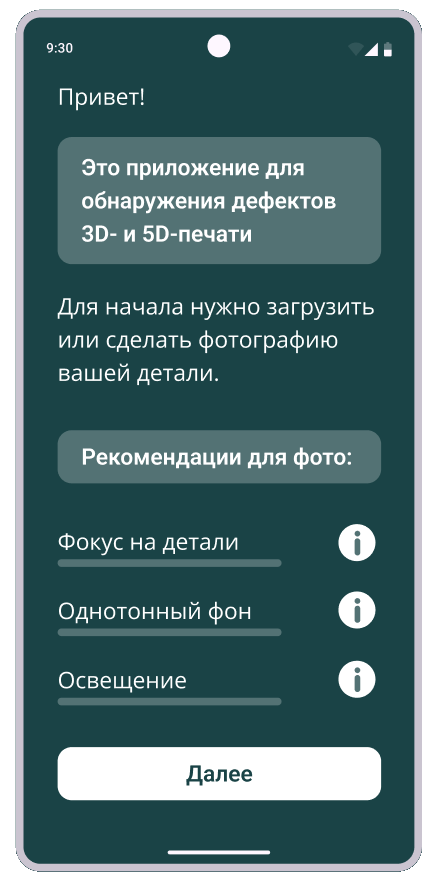
\includegraphics[width=\hsize]{fig/1.png}
    \caption{Приветственная страница с рекомендациями}
    \label{fig:obuchenie}
  \end{minipage}
  \hfill
  \begin{minipage}[b]{0.45\hsize}
    \centering
    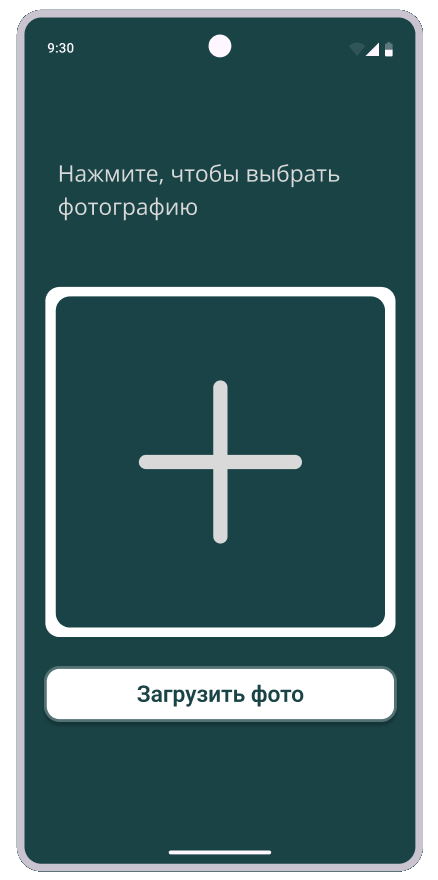
\includegraphics[width=\hsize]{fig/2.png}
    \caption{Страница загрузки фотографии}
    \label{fig:1}
  \end{minipage}
\end{figure}


\section{Обнаруженные недостатки выбранного подхода к распознаванию дефектов}

Изначально модель обучалась на 6 классах~-- это «спагетти», «паутина», деламинация, искревление геометрии, недоэкструзия и перегрев. Во время проведения поиска изображения для обучения нейросети возникла проблема, что в открытом доступе количество данных для одних классов значительно больше, чем для других. Например, найти качественные изображения с дефектом «спагетти» оказалось намного проще, чем для перегрева. После этапа формирования датасета получилось следующее соотношение: 1 класс~-- «спагетти»~-- 35~\%, 2 класс~-- «паутина» -- 20~\%, 3 класс~-- деламинация -- 10~\%, 4 класс~-- недоэкструзия~-- 15~\%, 5 класс~-- искревление геометрии~-- 10\%, 6 класс~-- перегрев~-- 10~\%. Процентное соотношение является приблизительным, поскольку в процессе создания аннотаций некоторые изображения были исключены.
График соотношения размеров классов от общего числа изображений представлен на рисунке \ref{fig:123456}.

\begin{figure}[h!]
\begin{center}
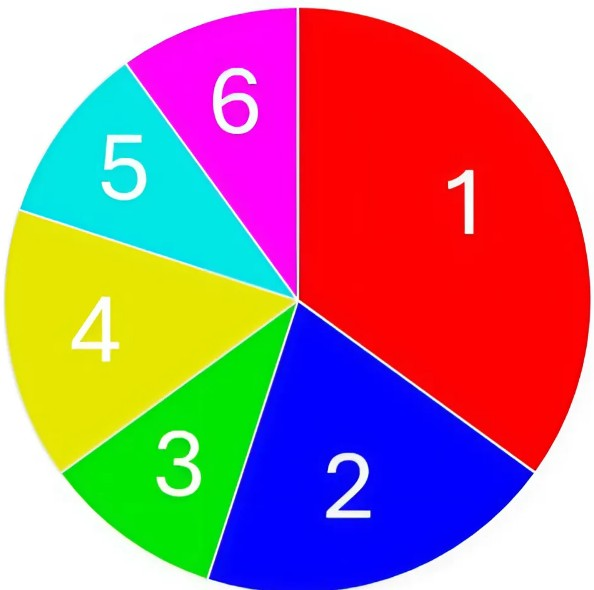
\includegraphics[width=0.4\hsize]{fig/123456.jpeg}
\caption{График соотношения размеров классов от общего числа изобра
жений}\label{fig:123456}
\end{center}
\end{figure}

Равномерное распределение классов в наборе данных критически важно для корректного обучения нейросети, поскольку дисбаланс может привести к значительному снижению точности предсказаний.

По графику заметно, что класс «спагетти» является самым большим, но это обусловлено тем, что дополнительным фактором, влияющим на размер класса, является его высокая вариативность. В отличие от других типов дефектов, «спагетти» может иметь широкий спектр визуальных проявлений: от единичных вытянутых нитей до плотных скоплений спутанного материала. Эта особенность усложняет процесс классификации, поскольку для эффективного распознавания необходимо учесть множество возможных конфигураций дефекта.

С другой стороны, класс делеминации составляет всего лишь 10~\% от общего объема изображений, но этого хватило для того, чтобы научить нейросеть достаточно хорошо находить этот дефект. Проблема возникает в том, что добиться того, чтобы нейросеть отличала делеминацию от недоэкструзии, так и не получилось.

Сложность в разграничении этих классов заключается в том, что оба дефекта могут проявляться визуально схожим образом. 

Особенно сложной ситуация становится в случае, когда недоэкструзия развивается горизонтально относительно стола 3D-принтера. Деламинация представляет собой расслоение, возникающее из-за недостаточной адгезии между слоями. Визуально это выражается в наличии разрывов или отслоений, расположенных горизонтально. Недоэкструзия же связана с нехваткой подаваемого материала, что приводит к появлению участков с уменьшенной толщиной слоя или разрывами в структуре. При вертикальном проявлении недоэкструзия выглядит как истончение стенок или неравномерное наполнение, что делает ее относительно легко отличимой. Однако при горизонтальной недоэкструзии, когда слой формируется с недостаточным количеством материала, он может напоминать деламинацию по внешнему виду, создавая разрывы, схожие с отслоением.

Исходя из этой проблемы, было решено на данном этапе оставить только дефект деламенации. Исключение недоэкструзии из набора позволило увеличить точность обнаружения деламенации. В дальнейшем возможно повторное введение класса «недоэкструзия».

На рисунках \ref{fig:nedo} и \ref{fig:delam} продемонстрирована схожесть дефектов недоэкструзии и деламенации, что увеличивает ошибку
\begin{figure}[h!]
  \begin{minipage}[b]{0.45\hsize}
    \centering
    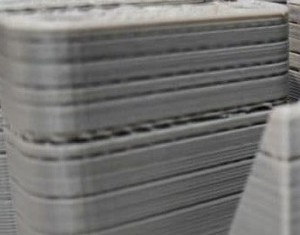
\includegraphics[width=\hsize]{fig/nedo.jpg}
    \caption{Дефект недоэкструзии на детали}
    \label{fig:nedo}
  \end{minipage}
  \hfill
  \begin{minipage}[b]{0.45\hsize}
    \centering
    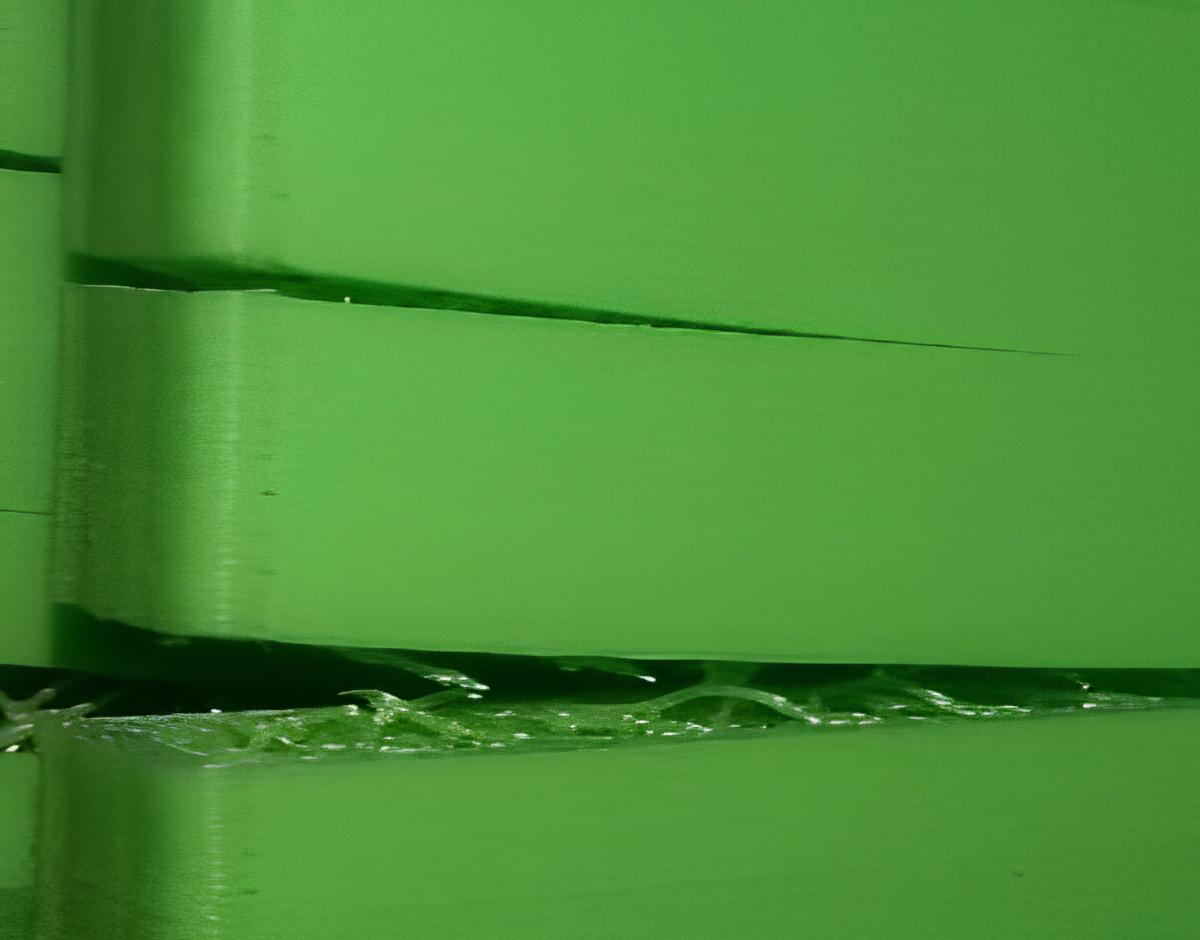
\includegraphics[width=\hsize]{fig/delam.jpg}
    \caption{Дефект деламенации на детали}
    \label{fig:delam}
  \end{minipage}
\end{figure}

Класс с дефектом перегрева, также пришлось удалить из набора из-за недостаточного количества и качества обучающих материалов. В конечном итоге осталось 4 класса.

Оценка точности работы нейросети требует использования специальных метрик, которые позволяют измерить качество предсказаний. Для объективной оценки используется показатель средней точности по классам при пороговом значении 0.5 (Average Precision by Class at IoU 0.5), сокращенно mAP50.

Данный показатель основан на метрике пересечения по объединению (Intersection over Union, IoU), которая измеряет степень совпадения предсказанной области с реальной. Если значение IoU превышает 0.5 (то есть пересечение составляет не менее 50~\% от общей площади двух областей), предсказание считается успешным.

Средняя точность (AP, Average Precision) рассчитывается для каждого класса отдельно и определяется как площадь под кривой, построенной по зависимости между точностью (Precision~-- доля корректных предсказаний среди всех найденных объектов) и полнотой (Recall~-- доля правильно найденных объектов среди всех существующих в данных).

Средняя средняя точность (mAP, Mean Average Precision)~-- это усредненное значение AP по всем классам. Показатель mAP50 учитывает только предсказания с IoU~$\geq$ 0.5 и используется в качестве базового критерия для оценки качества детекции. Чем выше его значение, тем точнее модель распознает дефекты, не требуя при этом строгого совпадения предсказанных и реальных границ.

Таким образом, точность по классам следующая: «спагетти»~-- 48~\%, «паутина»~-- 28~\%, деламинация~-- 31~\%, искревление геометрии~-- 31~\%.

Графики динамики ключевых метрик в процессе обучения нейросети представлены в приложении \ref{fig:1results} и \ref{fig:2results}. На всех графиках по оси X отложены итерации (эпохи) обучения, что показывает, как изменяются метрики со временем. По оси Y — значения соответствующих метрик: потерь, точности, полноты и средней точности.

Синяя линия — реальные измеренные значения метрик на каждой итерации обучения. Она имеет значительные колебания, так как значения метрик могут изменяться от набора данных, на каждом шаге.

Красная пунктирная линия~-- сглаженный тренд этих значений, который показывает общую тенденцию изменения метрик и помогает лучше понять, как модель обучается в целом.

Потери на классификации (class loss)~--  насколько хорошо модель различает классы. В начале обучения потери высокие, но со временем снижаются. Модель постепенно обучается правильно определять классы дефектов.

Потери на определении границ объектов (box loss)~-- точность определения границ дефектов. Видно, что этот показатель имеет тенденцию к росту, что говорит о проблемах с определениями границ дефектов.

Потери на обнаружении объектов (obj loss)~-- отражает, насколько хорошо модель определяет наличие дефекта. По графику виден рост, но колебания указывают на нестабильность.

Точность предсказаний (precision)~-- показывает долю правильно предсказанных дефектов среди всех обнаруженных. Значение постепенно увеличивается, значит точность растет.

Полнота предсказаний (recall)~-- измеряет, насколько полно модель находит дефекты. В начале обучения значение низкое, но затем постепенно увеличивается, что указывает на улучшение способности модели находить все дефекты в изображениях.

Средняя точность по классам при IoU~$\geq$ 0.5 (mAP)~-- характеризует общий уровень точности модели при небольших отклонениях в границах.

Средняя точность по классам при IoU от 0.5 до 0.95 (mAP 50 95)~-- показывает среднее значение точности модели по всем классам при разных значениях порога пересечения по объединению. Его значения остаются значительно ниже, чем у mAP50, что говорит о том, что при высоких значениях IoU модель испытывает трудности с точным определением границ дефектов.

Графики показывают, что модель постепенно обучается, ошибки классификации снижаются, точность и полнота предсказаний растут, но потери при обнаружении объектов и границ указывают на проблемы. Разница между mAP50 и mAP5095 говорит о том, что модель пока неточно определяет границы дефектов.

\section{Результат разработки и возможные методы улучшения работы приложения}

В результате работы удалось распознать четыре вида дефектов. Основной трудностью было различие между дефектами деламинации и недоэкструзии. Несмотря на аннотирование данных, нейросеть продолжала путать эти типы дефектов, особенно при горизонтальном проявлении недоэкструзии. Для повышения точности распознавания было решено временно исключить класс недоэкструзии из набора данных.

При тестировании приложения были обнаружены проблемы с обработкой малоразмерных изображений на серверной части. Для решения проблемы было внедрено автоматическое увеличение изображений до минимального рабочего разрешения в 800 на 800 пикселей. Результат обработки изображения и вывод списка дефектов представлен на рисунке \ref{fig:find}.

\begin{figure}[h!]
\begin{center}
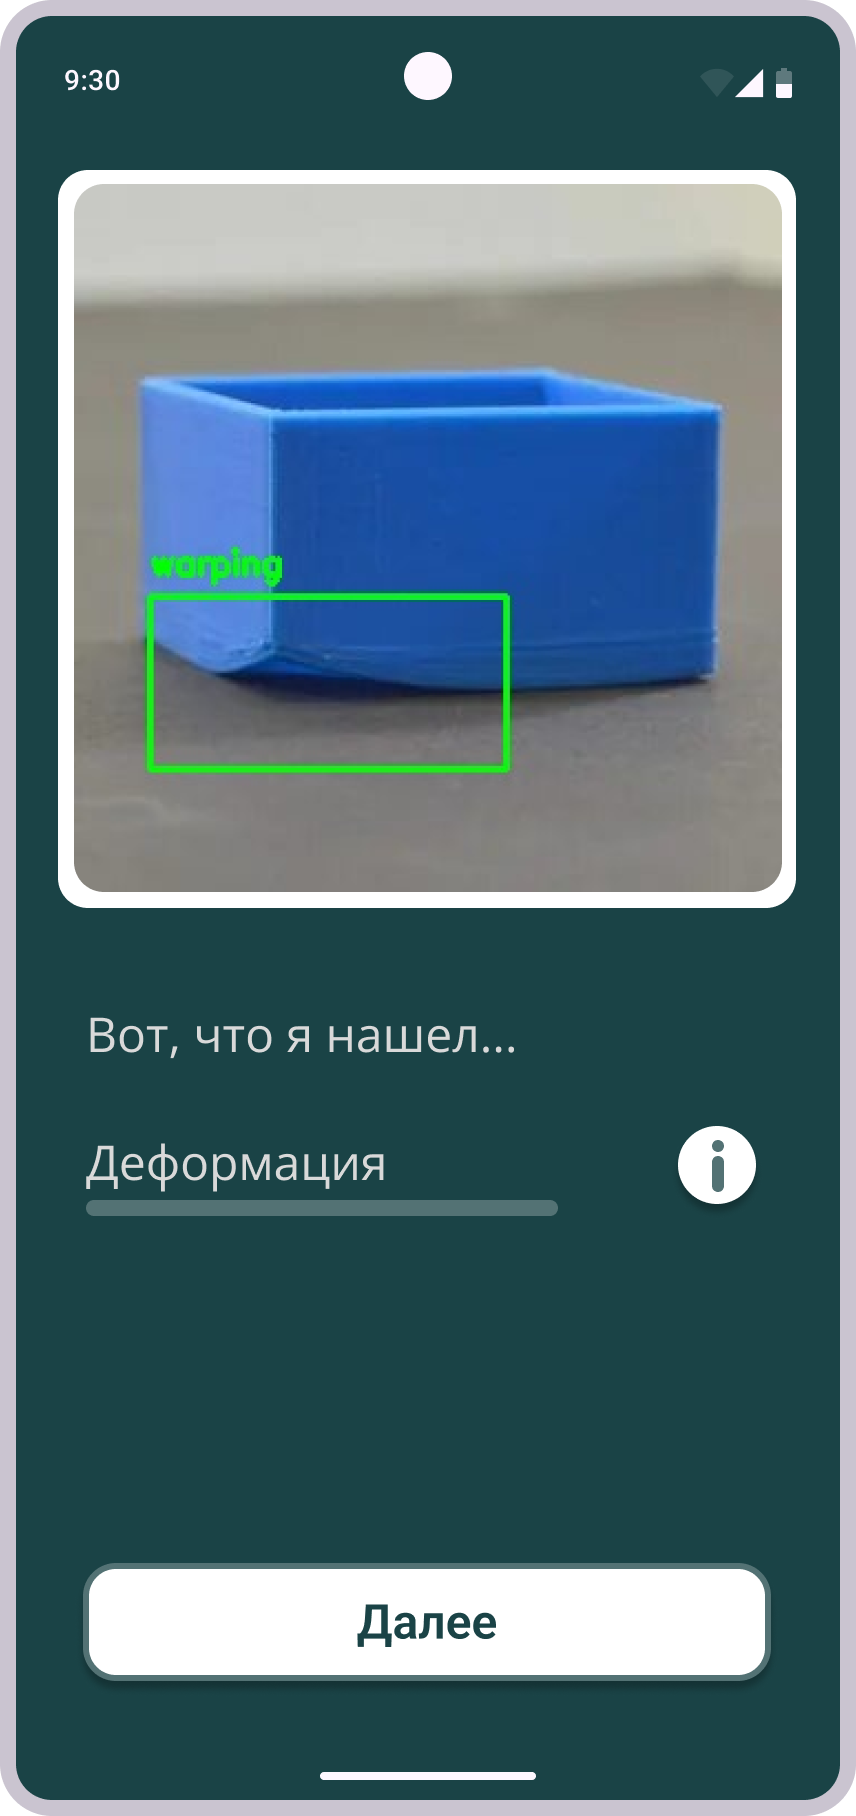
\includegraphics[width=0.4\hsize]{fig/find.png}
\caption{Экран с найденными ошибками и аннотированным изображением}\label{fig:find}
\end{center}
\end{figure}

Для тестирования качества распознавания дефектов были загружены изображения разной степени сложности. Анализируя полученные результаты распознавания дефектов, можно прийти к выводу, что даже на изображениях низкого качества нейросеть способна обнаружить дефекты с такой же точностью, как и на более чётком ее варианте, что означает эффективность проведенной аугментации.

Одна из главных проблем задачи заключается в том, что нейросети не всегда удается интерпритировать геометрию обьекта, чтобы определить на нем дефект. Часто явный дефект деламинации не распознавался из-за того, что на изображении была видна внутренняя геометрия объекта. Из-за этого нейронная сеть не могла с достаточной точностью определить его тип.
Подобная проблема представлена в приложении на рисунке \ref{fig:HeCracking} и \ref{fig:cracking}.

Изначально модель обучалась на 6 классах~-- это «спагетти», «паутина», деламинация, искревление геометрии, недоэкструзия и перегрев. Эти недостатки являются одними из самых визуально отличимых в 3D-печати, что должно было значительно облегчить процесс обучения, но из-за сложной геометрии фигур и их многообразия задача оказалась довольно сложной и трудоёмкой. Модель была обучена на части этих классах и теперь способна обнаруживать аналогичные дефекты. Планируется расширить список классов, включив другие виды дефектов 3D-печати, чтобы повысить точность распознавания и эффективность модели.

Эту ситуацию может улучшить внедрение единой тестовой модели, призванной выявить как можно больше дефектов. Такой подход способен значительно повысить точность обнаружения, поскольку процесс обучения будет происходить не только на различных деталях, но и на этой тестовой модели. Подобные модели находятся в открытом доступе, что значительно облегчает процесс создания единой детали для выявления дефектов. В дополнение к этому, планируется внедрение специальных маяков, которые должны помочь нейросети более точно понимать, как и с какого ракурса была сделана фотография. Это может улучшить качество анализа и ускорить процесс выявления дефектов. Подобная модель представлена на рисунке \ref{fig:test}.

\begin{figure}[h!]
\begin{center}
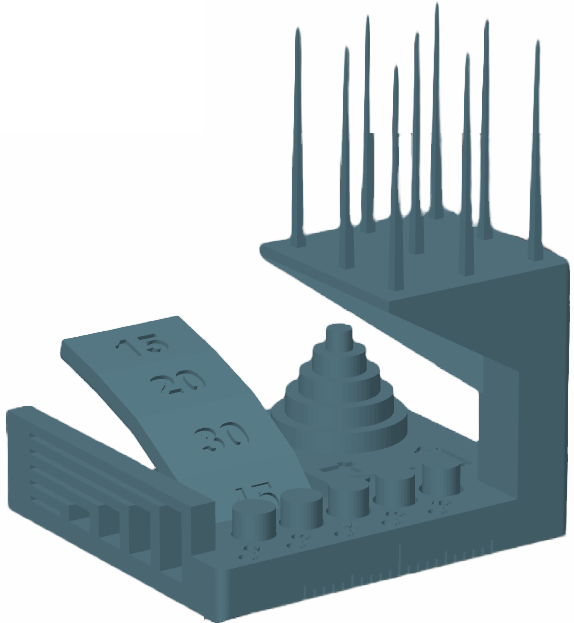
\includegraphics[width=0.55\hsize]{fig/Test.png}
\caption{Пример единой модели, печатаемой для выявления дефектов}\label{fig:test}
\end{center}
\end{figure}

\chapter{Реализация и экспериментальная проверка серверного контура обнаружения дефектов 3D-печати}

\section{Формирование набора данных, аннотирование и аугментация изображений}

Качество обнаружения дефектов в процессе~3D-печати напрямую зависит от качества исходного набора данных. Поэтому подготовка датасета выделена в отдельный инженерный этап с фиксированными правилами отбора, аннотирования и проверки разметки.

В данной работе датасет формируется преимущественно на основе собственных экспериментальных печатей: не менее 80~\% кадров собираются на разработанной установке в реальных условиях эксплуатации. До 20~\% изображений добавляются из открытых источников для расширения вариативности сцен и повышения устойчивости модели. Такой баланс сохраняет привязку к целевой конфигурации принтера и снижает риск переобучения на узкий набор условий.

Сбор основной части данных автоматизирован на уровне рабочего контура печати. После запуска задания макрос \texttt{START\_PRINT} вызывает \texttt{\_TREED\_CAM\_START}, который через Moonraker (API-сервис обмена командами и телеметрией) запускает \texttt{treed\_cam\_session\_start}. Скрипт \texttt{session\_start.sh} создает каталог сессии в \texttt{/home/pi/treed/cam/prints}, записывает путь в маркерный файл \texttt{/tmp/treed\_cam\_session\_dir} и сохраняет стартовый кадр.

Дальнейшая съемка выполняется периодически в процессе печати. Макрос \texttt{\_TREED\_CAM\_TICK} вызывает \texttt{treed\_cam\_snapshot}, а \texttt{snapshot.sh} добавляет кадры в каталог активной сессии. Интервал задается параметром \texttt{snapshot\_interval} в \texttt{\_TREED\_PRINT\_DEFAULTS}; в базовой конфигурации используется \(120~\text{с}\) с нижним ограничением \(10~\text{с}\). После завершения задания макрос \texttt{END\_PRINT} выполняет \texttt{\_TREED\_CAM\_STOP} и закрывает сессию.

При отборе изображений исключаются дубли, кадры с критически низкой резкостью и примеры, где зона печати не позволяет однозначно интерпретировать состояние процесса. В набор включаются кадры с дефектами и кадры штатной печати без отклонений.

Аннотирование выполняется в Roboflow в формате ограничивающих прямоугольников. Для каждой аннотации контролируются точность границ, отсутствие дублирующих рамок и соответствие фактической области дефекта.

Критичными ошибками считаются завышенные ограничивающие рамки и перекрытие нескольких рамок на одном дефекте. На рисунках~\ref{fig:big} и~\ref{fig:Granitsi} показаны эти случаи.

На рисунке~\ref{fig:big} ограничивающая рамка существенно превышает реальную область дефекта. В рамку попадает значительная часть фона. Это искажает геометрию объекта и ухудшает обучение модели.

На рисунке~\ref{fig:Granitsi} несколько рамок размечают один и тот же дефект. Такая разметка создает дубли и формирует неоднозначные обучающие примеры. При накоплении подобных ошибок снижается устойчивость модели на проверочных данных.

\begin{figure}[h!]
  \begin{minipage}[b]{0.45\hsize}
    \centering
    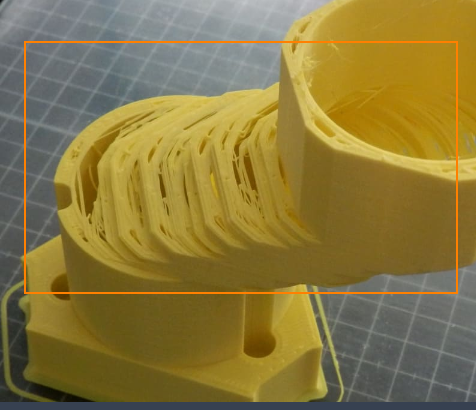
\includegraphics[width=\hsize]{fig/big.png}
    \caption{Слишком большие границы дефекта}
    \label{fig:big}
  \end{minipage}
  \hfill
  \begin{minipage}[b]{0.45\hsize}
    \centering
    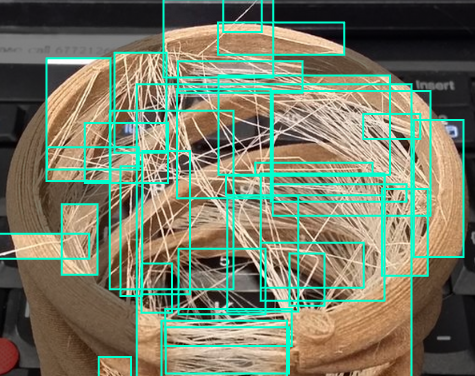
\includegraphics[width=\hsize]{fig/Granitsi.png}
    \caption{Границы дефектов перекрывают друг друга}
    \label{fig:Granitsi}
  \end{minipage}
\end{figure}

Качество разметки оценивается с учетом метрики Intersection over Union, которая отражает степень совпадения предсказанной и эталонной области. Неточные границы напрямую снижают значение этой метрики и ухудшают итоговое качество обнаружения. Поэтому автоматическая разметка используется только как вспомогательный шаг, а финальная валидация выполняется вручную.

После формирования исходного набора применяется аугментация изображений для повышения устойчивости к изменениям условий съемки. Используются преобразования яркости, контраста, умеренный шум и небольшие геометрические изменения, которые не разрушают структуру дефекта. Далее датасет разделяется на обучающую, валидационную и тестовую части с контролем представленности целевых дефектов.

В результате формируется датасет, ориентированный на реальные условия работы разработанного комплекса и пригодный для обучения серверной модели обнаружения дефектов. Принятые правила разметки и контроля качества снижают влияние шумовых факторов и повышают воспроизводимость экспериментов. На основе этого набора данных в следующем разделе рассматривается реализация серверного контура обработки визуальных данных.


\section{Реализация серверного контура обработки визуальных данных}

\section{Интеграция серверного анализа с контуром управления 3D-принтером}

\section{Результаты экспериментальных запусков, ограничения и направления развития}

\conclusion
В данной работе исследованы ключевые аспекты контроля качества 3D-печати методом FDM, включая анализ дефектов, их причины и методы устранения. Автоматизация процесса выявления дефектов с использованием машинного обучения и компьютерного зрения стала приоритетной задачей. Сравнительный анализ традиционных алгоритмов обработки изображений и нейросетевых моделей позволил определить наиболее эффективный подход к решению задачи.

В рамках работы разработано мобильное Android-приложение, предназначенное для автоматического распознавания дефектов, возникающих в процессе 3D-печати. Основной функцией приложения является анализ загружаемых изображений деталей и выявление на них возможных отклонений от нормы. Для реализации этой задачи была обучена сверточная нейронная сеть, способная детектировать наиболее распространённые дефекты, такие как «спагетти», «паутина», деламинация, геометрические искажения и другие. В процессе работы выполнен полный цикл подготовки модели: сбор и аннотирование изображений, аугментация данных, обучение нейросети и тестирование её на реальных примерах.

Кроме разработки алгоритмов детекции, была создана серверная часть на базе Python и Flask, обеспечивающая обработку изображений, передачу данных между мобильным клиентом и моделью, а также визуализацию результатов. После загрузки фотографии деталь проходит анализ, а на изображении отмечаются области с выявленными дефектами. Полученные результаты передаются обратно в приложение, где пользователь может просмотреть аннотированное изображение и подробное описание обнаруженных проблем.

Для эффективной работы модели была использована платформа Roboflow для аннотирования и аугментации данных. Для создания интерфейса и взаимодействия с сервером была выбрана среда разработки Android Studio. В ходе тестирования проводился анализ точности предсказаний нейросети, а также выявление возможных ограничений и их устранение.

% Новые компетенции (добавлены комментариями, источник: Kompetentsii_IVTm-24.txt)
% Учебная практика, проектно-технологическая практика
% УК-1 – Способен осуществлять критический анализ проблемных ситуаций на основе системного подхода, вырабатывать стратегию действий.
% УК-3 – Способен организовывать и руководить работой команды, вырабатывая командную стратегию для достижения поставленной цели.
% ПК-4 – Способен проектировать сложные пользовательские интерфейсы.
% ПК-5 – Способен разрабатывать требования и проектировать программное обеспечение.
% ПК-6 – Способен разрабатывать пользовательские документы, а также стандартные технические документы на основе предоставленного материала.

При выполнении данной работы были освоены следующие компетенции:

УК-2 Способен определять круг задач в рамках поставленной цели и выбирать оптимальные способы их решения, исходя из действующих правовых норм, имеющихся ресурсов и ограничений. При выполнении работы были определены ключевые задачи и проанализированы способы их решения, проведено тщательное их сравнение и выбран наилучший подход.

УК-4 Способен осуществлять деловую коммуникацию в устной и письменной формах на государственном языке Российской Федерации и иностранном(ых) языке(ах). Во время выполнения работы осуществлялась коммуникация с научным руководителем и коллегами в устной и письменной форме, что соответствует компетенции.

УК-6 Способен управлять своим временем, выстраивать и реализовывать траекторию саморазвития на основе принципов образования в течение всей жизни. Разработка приложения потребовала планирования работы, распределения задач и изучения новых подходов в области машинного обучения и компьютерного зрения.

ОПК-1 Способен применять естественнонаучные и общеинженерные знания, методы математического анализа и моделирования, теоретического и экспериментального исследования в профессиональной деятельности. В процессе работы использованы принципы машинного обучения, компьютерного зрения и программирования для обработки изображений и распознавания дефектов.

ОПК-3 Способен решать стандартные задачи профессиональной деятельности на основе информационной и библиографической культуры с применением информационно-коммуникационных технологий и с учетом основных требований информационной безопасности. Во время выполнения работы были использованы различные информационно-коммуникационные технологии и ресурсы для поиска и анализа необходимой информации по теме работы.

ОПК-5 Способен инсталлировать программное и аппаратное обеспечение для информационных и автоматизированных систем. В ходе работы осуществлена настройка среды разработки, установка и конфигурация программного обеспечения для работы с нейросетью и API Roboflow.

ПК-1 Способен проводить анализ научной литературы, принимать участие в научно-исследовательских и опытно-конструкторских работах с использованием компьютерного моделирования, современных методов обработки информации и оформлять полученные результаты в виде отчетов, презентаций и докладов. В процессе выполнения работы проведён анализ научной литературы, применение полученных знаний на практике и использование современных методов обработки информации. Результат работы представлен в виде отчёта.

ПК-2 Способен производить анализ требований к программному обеспечению и проектировать программный продукт. В ходе работы сформулированы требования к функционалу приложения, спроектирована его архитектура и реализована серверная и клиентская часть для обработки изображений.

ПК-3 Способен создавать, модифицировать и сопровождать информационные системы. Разработано и протестировано приложение, интегрированное с нейросетью для детекции дефектов в 3D-печати, а также обеспечена его оптимизация для работы с различными устройствами.

\printbibliography[heading=bibintoc]
\include{Bib.bib}
\chapter*{Ход выполнения практики}
\addcontentsline{toc}{chapter}{Ход выполнения практики}

\section*{Задания и отметки о выполнении}

\task{Написать обзор по предметной области исследования,
основываясь на научной, учебной и учебно-методической литературе, как на русском, так
и на английском языках. Необходимо использовать современную литературу на английском и русском языках по тематике научно-исследовательской работы, поиск которой можно осуществлять по библиографическим базам Scopus, WoS, elibrary, ResearchGate, ADS, ЭБС Лань и др.}

\task{Изучить особенности FDM-печати и типы возможных дефектов, возникающих в процессе.}

\task{Разработать удобный и интуитивно понятный пользовательский интерфейс приложения.}

\task{Обучить нейронную сеть распознаванию дефектов 3D-печати на основе изображений изделий.}

\task{Реализовать функционал приложения, включая загрузку данных, их обработку и визуализацию результатов.}

\task{Подготовить отчет по практике в соответствии с компетенциями направления 09.04.01 Информатика и вычислительная техника.}

\task{Создать презентацию в соответствии с данным отчетом и устный доклад для публичной защиты.}

\clearpage
\section*{Отзыв о работе обучающегося}

В ходе прохождения производственной практики, научно-исследовательской работы Ешенко Даниил Ярославович выполнил поставленные ему задачи, а именно изучил особенности FDM-печати и типы возможных дефектов, возникающих в её процессе, спроектировал интуитивно понятный пользовательский интерфейс мобильного приложения, а также обучил нейронную сеть распознаванию дефектов 3D-печати и реализовал функционал приложения, включая загрузку данных, их обработку и визуализацию результатов. По итогам работы было создано мобильное приложение на базе Android для обнаружения дефектов 3D-печати. Считаю, что его работа заслуживает положительной оценки.
\progressapprov
\appendix
\chapter{Схема электрической коммутации компонентов 3D-принтера}\label{app:commutation_scheme}

Наглядная схема электрической коммутации компонентов принтера приведена на рисунке~\ref{fig:appendix_commutation_scheme}.

\begin{figure}[h!]
\begin{center}
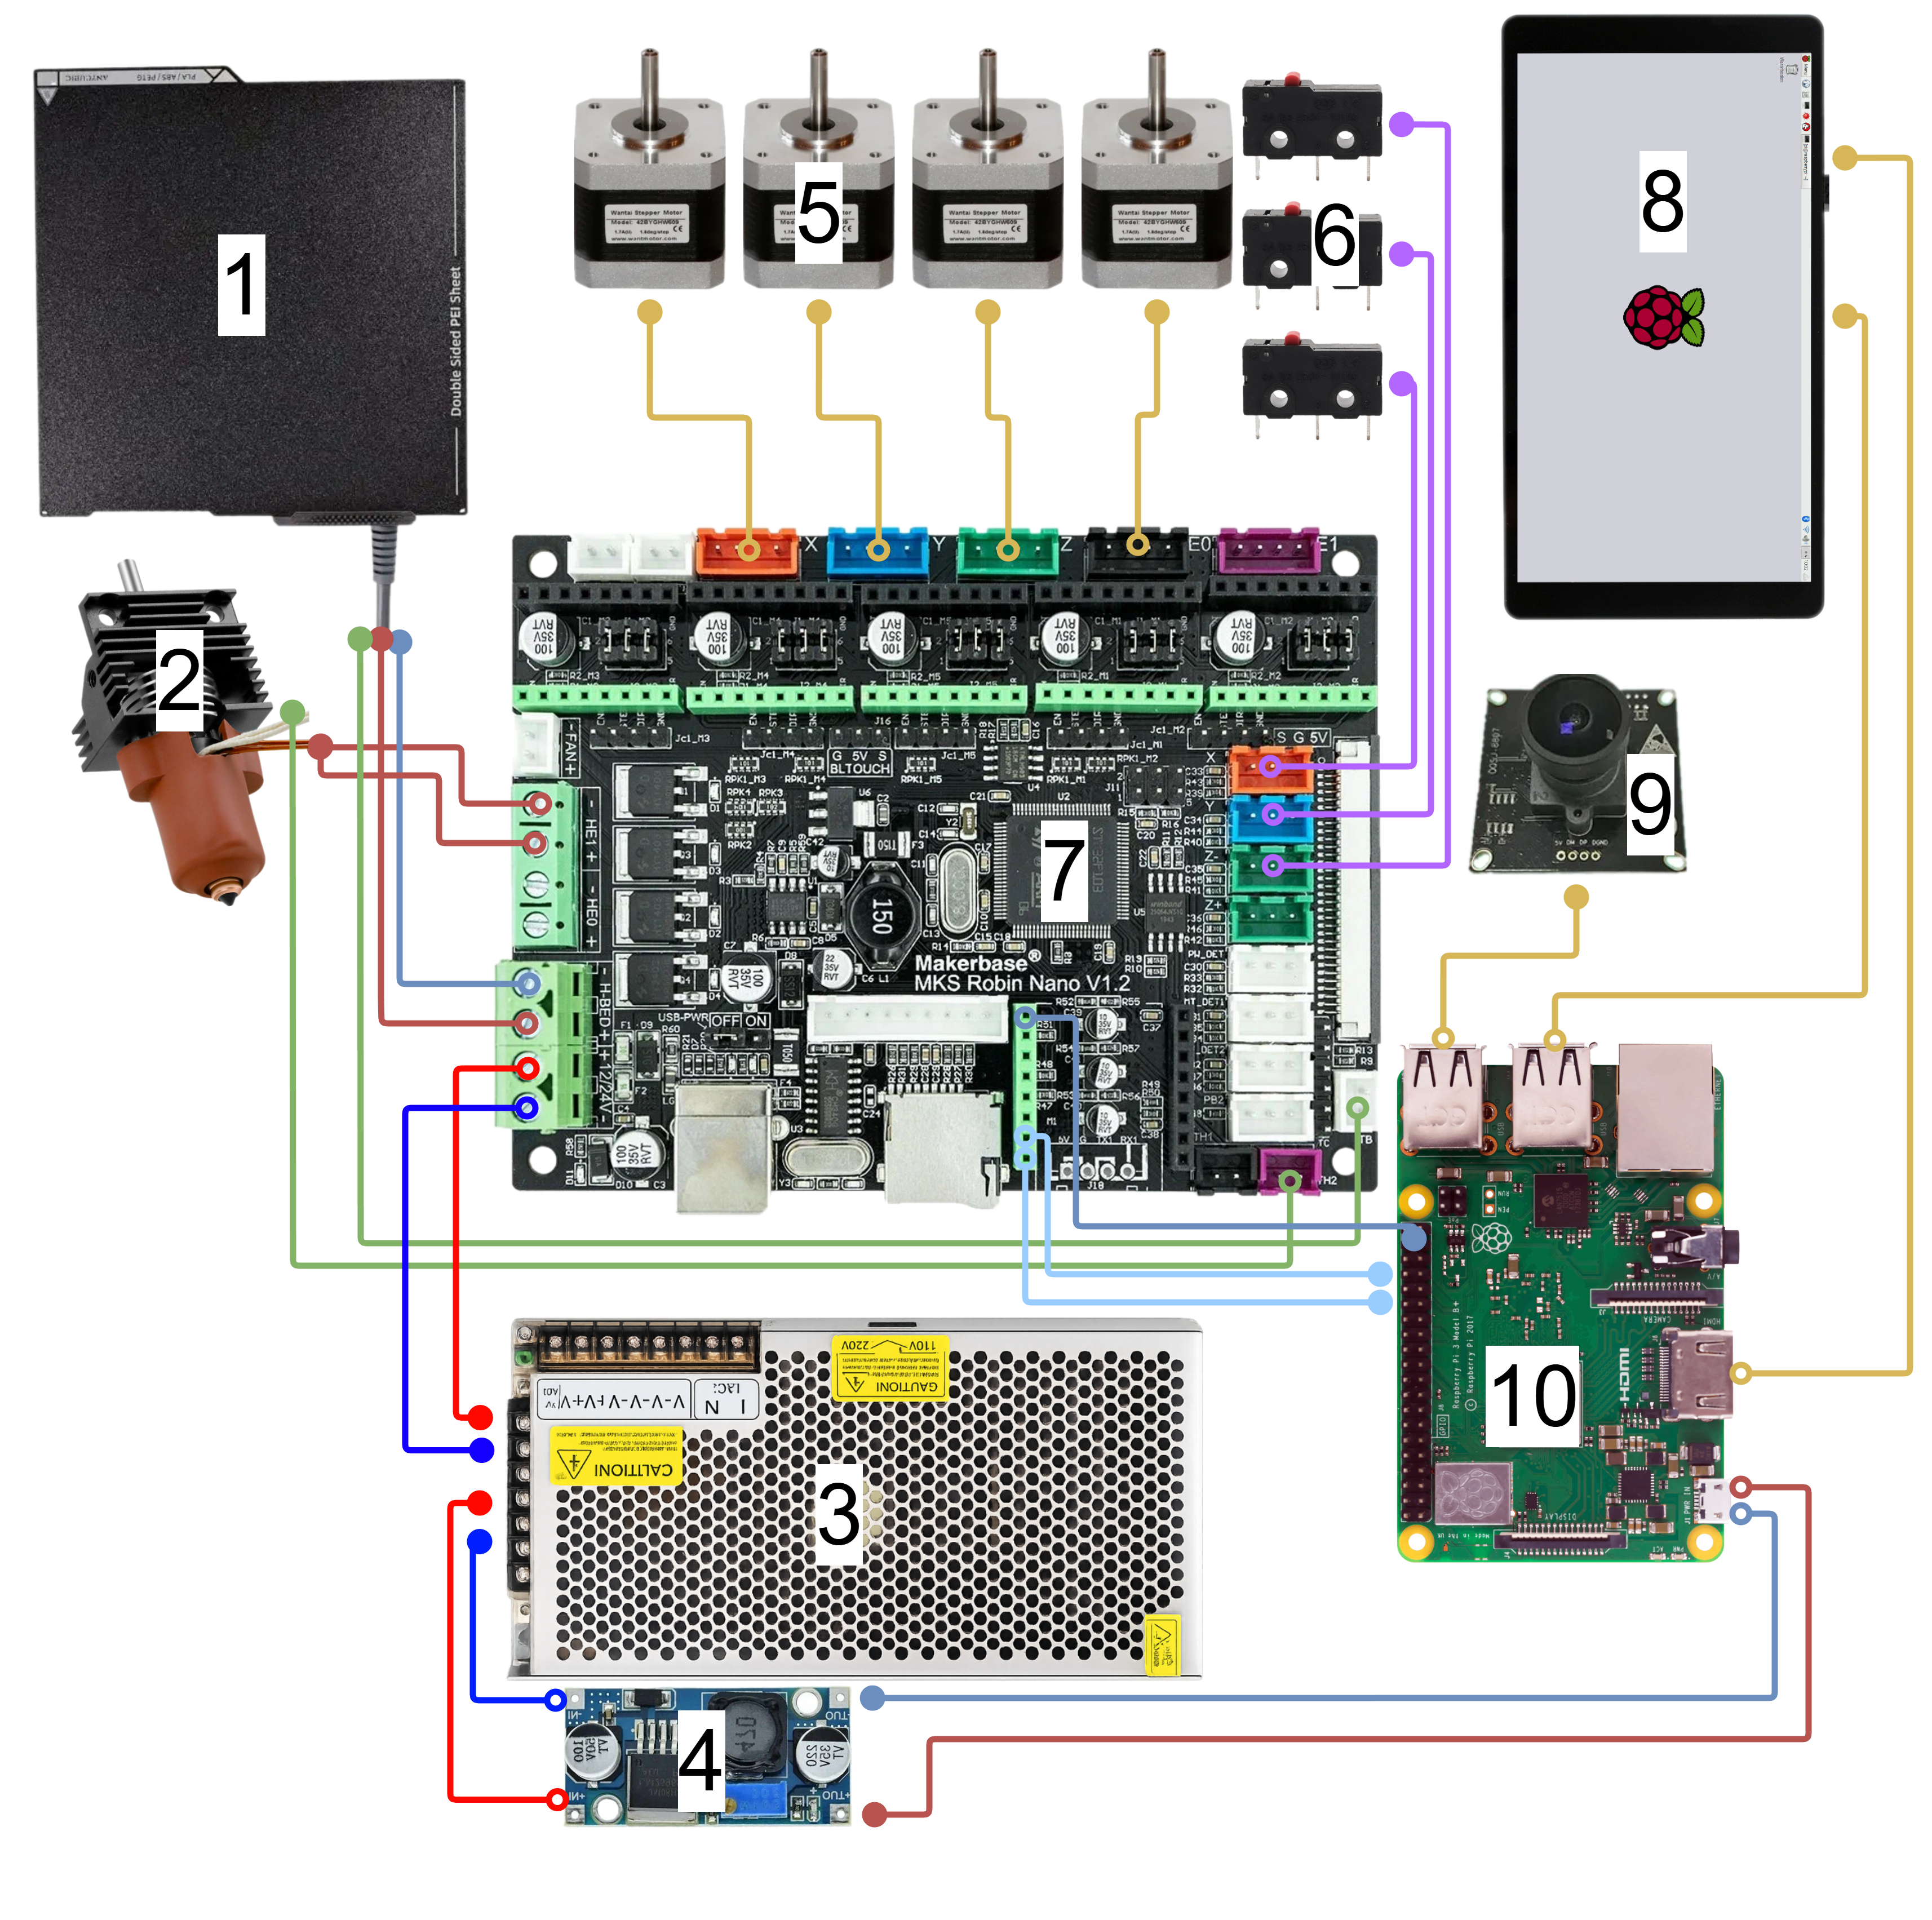
\includegraphics[width=\hsize]{fig/commutation_diagram_nir2.png}
\caption{Схема электрической коммутации компонентов 3D-принтера}\label{fig:appendix_commutation_scheme}
\end{center}
\end{figure}

Описание подключений по позициям схемы:

\begin{itemize}
\item Позиция 1 — нагреваемый стол. Нагревательный стол подключается к плате MKS Robin Nano~1.2 как силовая нагрузка контура стола. В актуальной конфигурации прошивки это соответствует блоку \texttt{[heater\_bed]} с каналом управления нагревом \texttt{heater\_pin: PA0}. Температурный контроль стола реализован через отдельный термодатчик, подключенный к измерительному входу платы; в профиле задано \texttt{sensor\_type: NTC100K\_B3950} и \texttt{sensor\_pin: PC0}. Для безопасной эксплуатации заданы программные ограничения и проверка набора температуры (\texttt{max\_temp: 120}, \texttt{max\_power: 1.00}, блок \texttt{[verify\_heater heater\_bed]}).

\item Позиция 2 — нагреватель и термистор хотэнда. Нагреватель хотэнда подключен к плате MKS Robin Nano~1.2 как отдельный силовой канал экструдера; в актуальном профиле это блок \texttt{[extruder]} с \texttt{heater\_pin: PB0}. Термодатчик хотэнда подключен к отдельному измерительному входу платы и описан как \texttt{sensor\_type: NTC100K\_B3950} с \texttt{sensor\_pin: PC1}. Для защиты от нештатных режимов заданы температурные и технологические ограничения (\texttt{max\_temp: 280}, \texttt{max\_power: 1.0}, \texttt{min\_extrude\_temp: 170}).

\item Позиция 3 — блок питания. Блок питания работает от сети 220~В и формирует выходную шину 24~В для низковольтной части принтера. В данной конфигурации напрямую к выходу блока питания подключены только плата MKS Robin Nano~1.2 и понижающий преобразователь DC-DC. Подключение остальных нагрузок выполняется через плату MKS.

\item Позиция 4 — понижающий преобразователь DC-DC. Понижающий преобразователь получает питание от шины 24~В и формирует стабилизированную линию 5~В для низковольтной подсистемы. К выходу преобразователя подключены Raspberry Pi~3B, USB-камера Sonix USB 2.0 и экран. Такое разделение контуров позволяет питать хостовые устройства от отдельной линии 5~В и не подключать их напрямую к выходам платы MKS Robin Nano~1.2.

\item Позиция 5 — шаговые двигатели и драйверы TMC2209. Подключение двигателей выполнено через моторные разъемы платы MKS Robin Nano~1.2, обозначенные в даташите как \texttt{X}, \texttt{Y}, \texttt{Z1}, \texttt{E0}, \texttt{E1}. В текущей конфигурации задействованы \texttt{X}, \texttt{Y}, \texttt{Z1} и \texttt{E0}; разъем \texttt{E1} не используется. Для этих каналов установлены драйверы TMC2209, при этом в профиле прошивки задано \texttt{microsteps: 16}, а секции \texttt{[tmc*]} отсутствуют, что соответствует автономному режиму работы драйверов.

\item Позиция 6 — концевые выключатели. Концевые выключатели осей X, Y и Z подключены к сигнальным входам платы MKS Robin Nano~1.2 и используются для выполнения процедуры фиксации базовых координат принтера. В профиле прошивки они заданы как \texttt{endstop\_pin: \^PA15} для оси X, \texttt{endstop\_pin: \^PA12} для оси Y и \texttt{endstop\_pin: \^PA11} для оси Z. Корректная работа концевых выключателей влияет на точность базирования и предотвращает выход механики за допустимые пределы перемещения.

\item Позиция 7 — плата управления MKS Robin Nano~1.2. Плата является центральным узлом коммутации и управления: на нее подается питание 24~В, к ней подключаются исполнительные и измерительные цепи принтера, а также линия связи с Raspberry Pi. На уровне прошивки MKS работает как MCU в контуре Klipper, выполняя обработку команд реального времени для двигателей, нагревателей и датчиков. В текущей конфигурации обмен с хостом выполняется по UART, что соответствует принятой архитектуре управления в проекте.

\item Позиция 8 — AMOLED-экран. Экран подключен к Raspberry Pi по интерфейсу HDMI для вывода изображения и по USB для работы сенсорного ввода. Такая схема разделяет видеоканал и канал передачи событий касания, что обеспечивает корректную работу локального интерфейса управления.

\item Позиция 9 — камера. Камера подключена к Raspberry Pi по USB и используется как источник видеоданных для наблюдения за зоной печати. Далее видеопоток передается в программный контур мониторинга и используется для обнаружения отклонений в процессе 3D-печати.

\item Позиция 10 — Raspberry Pi~3B. Raspberry Pi является хост-узлом контура управления: на нем работают сервисы Klipper и Moonraker, а также подсистема видеомониторинга. Сигнальная связь с платой MKS Robin Nano~1.2 выполнена по UART через контактный разъем GPIO Raspberry Pi и разъем WiFi-UART платы MKS: \texttt{GPIO14 / pin 8 (TX) -> PA10 (RX)}, \texttt{GPIO15 / pin 10 (RX) -> PA9 (TX)}, общий провод \texttt{GND -> GND}. В текущей конфигурации проекта именно этот UART-канал используется как основной рабочий канал связи.
\end{itemize}

\chapter{Последовательность этапов сценария развертывания}\label{app:loader_steps}

В данном приложении приведен полный перечень шагов shell-сценария \texttt{loader.sh}, используемого для воспроизводимого развертывания программного контура в репозитории \texttt{treed-mainshellOS}. В рамках сценария используются два типа этапов: \texttt{required} (ошибка прерывает процесс) и \texttt{optional} (ошибка фиксируется в журнале, после чего выполнение продолжается). Под развертыванием в данном контексте понимается автоматизированная подготовка системы к рабочему состоянию, включая настройку загрузки, сервисов и runtime-конфигурации печати.

\begin{enumerate}
\item \texttt{check-env.sh} --- выполняет базовую валидацию окружения запуска: проверяет права, обязательные переменные контракта лоадера и доступность целевого домашнего каталога пользователя.
\item \texttt{detect-rpi.sh} --- определяет модель Raspberry Pi и реальные boot-пути, после чего экспортирует их для последующих шагов, чтобы исключить расхождения между вариантами разметки boot-раздела.
\item \texttt{timezone-sync.sh} --- синхронизирует часовой пояс и состояние службы времени по протоколу Network Time Protocol (NTP), что требуется для корректной временной метки логов и событий.
\item \texttt{maintenance-stop.sh} --- переводит систему в режим обслуживания: останавливает ключевые runtime-сервисы перед изменением конфигурации и предотвращает конфликты доступа к файлам.
\item \texttt{packages-core.sh} --- устанавливает базовые системные зависимости и выполняет санитарные проверки критичных утилит, которые используются в последующих этапах сценария.
\item \texttt{boot-hdmi-config.sh} --- приводит к целевому виду блок настроек видеовыхода High-Definition Multimedia Interface (HDMI) и параметр \texttt{gpu\_mem} в \texttt{config.txt}, сохраняя управляемую и идемпотентную структуру файла.
\item \texttt{rpi-uart-config.sh} --- подготавливает канал Universal Asynchronous Receiver-Transmitter (UART) для связи с микроконтроллерным узлом (MCU): нормализует \texttt{enable\_uart}, отключает конфликтующую serial-console и применяет правила доступа к UART-устройствам.
\item \texttt{plymouth-theme-install.sh} --- устанавливает тему Plymouth (подсистема графической заставки загрузки Linux), проверяет полноту ее файлов и назначает тему по умолчанию.
\item \texttt{plymouth-initramfs.sh} --- пересобирает \texttt{initramfs} (образ ранней инициализации Linux) с установленной темой загрузки и копирует актуальный образ в boot-раздел.
\item \texttt{plymouth-initramfs-config.sh} --- вносит в \texttt{config.txt} согласованную строку подключения \texttt{initramfs} и отключает конфликтующие автоматические механизмы при их наличии.
\item \texttt{plymouth-cmdline.sh} --- нормализует параметры kernel command line (\texttt{cmdline}), удаляет конфликтные токены и формирует целевой набор параметров загрузки в фиксированном порядке.
\item \texttt{plymouth-systemd.sh} --- согласует состояние systemd-юнитов, связанных с консолью и завершением заставки загрузки, чтобы поведение при старте системы оставалось предсказуемым.
\item \texttt{klipper-sync.sh} --- синхронизирует дерево конфигураций Klipper из репозитория в промежуточный каталог (\texttt{staging}) с нормализацией владельца файлов.
\item \texttt{klipper-profiles.sh} --- применяет профиль RN12 и вычисляет корректный serial-путь MCU для выбранного транспорта (\texttt{usb} или \texttt{uart}), после чего идемпотентно обновляет \texttt{mcu\_rn12.cfg}.
\item \texttt{klipper-core.sh} --- переносит конфигурацию из \texttt{staging} в рабочий каталог (\texttt{runtime}), учитывая режим развертывания (\texttt{clean} или \texttt{preserve}) и сохранение локальных переопределений при необходимости.
\item \texttt{klipper-anti-shutdown.sh} --- диагностирует состояние Klipper после раскладки и при обнаружении аварийного состояния MCU выполняет контролируемый \texttt{FIRMWARE\_RESTART}.
\item \texttt{moonraker-config.sh} --- развертывает конфигурацию Moonraker (API-сервис взаимодействия с Klipper), выполняет валидацию и перезапуск с проверкой готовности сервиса.
\item \texttt{crowsnest-webcam.sh} (\texttt{optional}) --- настраивает видеоконтур через crowsnest (служба публикации потока камеры), подготавливает webcam-фрагменты конфигурации и выполняет проверки доступности устройства.
\item \texttt{treed-cam.sh} --- разворачивает runtime-скрипты камерного контура TreeD, нормализует права и исполняемость shell-файлов для дальнейшего использования в рабочем цикле.
\item \texttt{klipper-mainsail-theme.sh} --- выполняет синхронизацию темы пользовательского интерфейса Mainsail в runtime-конфигурацию.
\item \texttt{klipperscreen-install.sh} (\texttt{optional}) --- устанавливает и проводит первичную проверку KlipperScreen (локальный экранный интерфейс управления принтером).
\item \texttt{klipperscreen-theme.sh} (\texttt{optional}) --- разворачивает тему, шрифты и параметры языка для KlipperScreen, после чего перезапускает сервис для применения изменений.
\item \texttt{klipperscreen-integr.sh} (\texttt{optional}) --- применяет systemd override для корректной интеграции KlipperScreen в цепочку запуска и проверяет успешность перезапуска.
\item \texttt{maintenance-start.sh} --- завершает режим обслуживания и запускает required/best-effort сервисы с ожиданием перехода в рабочее состояние.
\item \texttt{verify.sh} --- выполняет финальную валидацию всего контура: проверяет boot-настройки, сервисы, serial-путь MCU, параметры UART/USB, состояние камеры и формирует итог pass/fail по результатам проверок.
\end{enumerate}


\end{document}
